%% Verze pro oboustranny tisk:
% Okraje: 
% (ale pozor, LaTeX si prida 1in)
\documentclass[10pt,a5paper]{article}
\usepackage[czech,english]{babel}
\usepackage[a5paper,margin=10mm]{geometry}
\newgeometry{top=20mm,bottom=20mm,right=15mm,left=15mm}
%\setlength\textwidth{102mm}
%\setlength\textheight{145mm}
%\setlength\oddsidemargin{0mm}
%\setlength\evensidemargin{0mm}
%\setlength\topmargin{0mm}
%\setlength\headheight{5mm}
%\setlength{\headheight}{15pt}
%\setlength{\parindent}{1cm}
\usepackage{pdfpages}
\usepackage{textcomp}

\usepackage[utf8]{inputenc}

\usepackage{bibentry}
\usepackage{url}
\usepackage[nottoc]{tocbibind}
\nobibliography*

\usepackage{titlesec}  %vzhled titulku prvni stranky kapitoly
%\let\footruleskip\undefined
\usepackage{fancyhdr}  %hlavicky stranek 

%% Ostatn� bal��ky
\usepackage{graphicx}
%\usepackage{amsthm} % for mathematical theorems, lemma, proof
\usepackage{amsmath} % for mathematical equation
\usepackage{amssymb} % for special symbols - blacktriangledown
%\usepackage{palatino} % font
%\usepackage{bookman} % another font
\usepackage[sc]{mathpazo} %palladio font
\usepackage[scaled]{helvet}
\usepackage{eulervm}

%\usepackage{setspace} % for linespacing
%\linespread{1.0}%\sin­glespac­ing %\onehalfspacing 
\usepackage[T1]{fontenc} %font encoding e.g. for czech characters
%\usepackage{diagbox} %diagonala v tabulce
%\usepackage{multirow} %viceradkove tabulky
%\usepackage[font=footnotesize]{caption} %velikost fontu v popisu
%\usepackage{etoolbox} %pro pozdejsi definici zpetne reference
%\usepackage[titletoc]{appendix} %appendices with names
%\usepackage{listings,multicol} % for code listings, multicolumned
%\lstset{% escape sequence inside listing
%  escapeinside={(*}{*)},%
%}
%\usepackage{dtsyntax} % for listings modelica
%\usepackage[version=3]{mhchem} % for writing chemical compounds and reaction
%\usepackage{siunitx} % formating numbers
%\renewcommand{\ttdefault}{pcr} % nicer font - courier in listing
\usepackage[unicode,colorlinks,backref=page]{hyperref}   % Musi byt za vsemi ostatnimi balicky
\hypersetup{pdftitle={Utilization of GRID in processing of medical information},
            pdfauthor={Tomáš Kulhánek},
            plainpages=false,
            urlcolor=blue,
            linkcolor=blue,
            citecolor=blue
            }

%\overfullrule=2cm %vyznacit na okraji, kde se nepodarilo zarovnat
%definice jak ma vypadat zpetna reference
%\makeatletter
%\patchcmd{\BR@backref}{\newblock}{\newblock(cited on p.~}{}{}
%\patchcmd{\BR@backref}{\par}{)\par}{}{}
%\renewcommand\bibentry[1]{\nocite{#1}{\frenchspacing
%     \@nameuse{BR@r@#1\@extra@b@citeb}}}
%\makeatother
\makeatletter
\def\@makechapterhead#1{
  {\parindent \z@ \raggedright \normalfont
   \Huge\bfseries \thechapter. #1
   \par\nobreak
   \vskip 10\p@
}}
\def\@makeschapterhead#1{
  {\parindent \z@ \raggedright \normalfont
   \Huge\bfseries #1
   \par\nobreak
   \vskip 10\p@
}}
\makeatother

\begin{document}
\shorthandoff{-} % fix problems with babel czech and includepdf chars '-' 
\pagenumbering{arabic} %first pages with roman numbering
\setcounter{page}{1}
%\lefthyphenmin=2
%\righthyphenmin=2
\pagestyle{empty} % title page without number
%\singlespacing 
%\sin­glespac­ing % 1.0 row space
\begin{center}
%\singlespacing 
\large
%\begin{tabular}{rl}
\textbf{\Large{Univerzita Karlova v Praze}}

\textbf{\Large{1.lékařská fakulta}} 

\textit{Charles University in Prague} 

\textit{1st Faculty of Medicine}
%\end{tabular}
\vfill
\normalsize
\begin{tabular}{rl}
Studijní obor:  & Biomedicínská informatika \\
\noalign{\vspace{-1mm}}
\textit{Study domain} & \textit{Biomedical informatics} \\
\end{tabular}

\vfill

{\Large Autoreferát dizertační práce}

\textit{\large Summary of the dissertation}

\centerline{\mbox{
\includegraphics[width=35mm]{img/logouk.jpg}

\includegraphics[width=35mm]{img/logolf1.jpg}}}

\vfill



% N�zev pr�ce p�esn� podle zad�n�
\textbf{\large Využití technologie GRID při zpracování medicínské informace}

\vspace{2mm}
\textit{\large Utilization of GRID technology in processing of medical information}
\vfill
{\Large Mgr. Tomáš Kulhánek}

% N�zev katedry nebo �stavu, kde byla pr�ce ofici�ln� zad�na
% (dle Organiza�n� struktury MFF UK)
% CESNET z.s.p.o., Institute of pathological physiology



\vfill

Praha 2015

\end{center}


%\frontmatter
%\onehalfspacing %1.5 row space
\newpage
\selectlanguage{czech}
%\normalsize
\begin{center}
\textbf{Doktorské studijní programy v biomedicíně}

\textit{Univerzita Karlova v Praze a Akademie věd České republiky}
\end{center}
\normalsize

\vspace{2mm}

Obor: Biomedicínská informatika
\vfill
Předseda oborové rady: Prof. RNDr. Jana Zvárová, DrSc.
\vfill

Školicí pracoviště: CESNET z.s.p.o., Ústav patologické fyziologie 1.LFUK
\vfill


Školitel:  Ing. Milan Šárek, CSc.
\vfill

Konzultant:  Doc. MUDr. Jiří Kofránek, CSc. 
\vspace{120mm}

Disertační práce bude nejméně pět pracovních dnů před konáním obhajoby zveřejněna
k nahlížení veřejnosti v tištěné podobě na Oddělení pro vědeckou činnost a zahraniční styky
Děkanátu 1. lékařské fakulty.


%
\newpage
\selectlanguage{english}

\begin{center}
\Large \textbf{Dedication}
\end{center} 
\vfill
\begin{center}
To my beloved children Karla and Matěj and my dearest lovely wife Marie,

without whom this work would not have been completed.
\end{center} 
\vfill
\newpage
\mbox{}
\newpage
\pagestyle{plain} % other pages with number
\begin{center}
\Large \textbf{Acknowledgements}
\end{center} 
I would like to express my gratefulness to my supervisor Ing. Milan Šárek, CSc. for his support and guidance throughout the beginning of my research. 
I would also like to thank the staff of association CESNET, especially Ing. Jiří Navrátil, CSc., who gave me an opportunity to work with computing resources connected via high speed academic network and to follow the development of the networking technologies. Further thanks go to the staff of METACENTRUM, department of CESNET, for giving support and access to powerful computing infrastructure for scientific purposes. I would like to thank to the staff of EGI.eu, who gave me an opportunity to be EGI Champion, selected users of scientific European grid-computing and cloud-computing infrastructure. This made me possible to meet the most inspiring people in the technology domain as well as scientific domain face to face. 

I would like to thank the fellows from Musical Acoustic Research Center of Academy of Performing Arts, especially RNDr. Marek Frič, PhD. and Ing. Zdeněk Otčenášek, Phd. for their inspiring atmosphere in the research domain of voice science. 

I would like to thank my colleagues from Laboratory of Biocybernetics and Computer Aided Teaching within Institute of Pathological Physiology including Mgr. Marek Mateják, Ing. Jan Šilar, Ing. Filip Ježek, Ing. Martin Tribula and MUDr. et Mgr. Pavol Privitzer, who provided me pleasure and inspiring atmosphere for my research and development work during the second part of my research. Especially, I would like to thank to my consultant Doc. MUDr. Jiří Kofránek, CSc. and a fellow MUDr. Stanislav Matoušek, PhD., who taught me the subject of medical physiology and who guided me within the topic of mathematical models and simulation of integrative physiology. Last but not least, thanks to Veronika Sýkorová, DiS and Klára Ulčová, DiS for their help with graphical schemas. 

The research projects were solved within the cooperation between association CESNET, First Faculty of Medicine of Charles University in Prague and Academy of Performing Arts in Prague and was partially supported by the project of Ministry of Education, Youth and Sport of the Czech Republic MSM6383917201, by the projects of Development Fund of CESNET 2009/361, 2010/384, 2011/423, 2011/431 and by the project of Ministry of Industry and Trade of the Czech Republic MPO FR-TI3/869.

\newpage
\mbox{}

%\pagestyle{plain} % other pages with number
%\mainmatter

\tableofcontents

\newpage
\section*{Abstrakt}
\addcontentsline{toc}{section}{Abstrakt (česky)}


%%% Povinn� informa�n� strana diserta�n� pr�ce

\vbox to 0.5\vsize{
\begin{center}
\Large \textbf{Abstrakt (česky)}
\end{center} 
\normalsize
\setlength\parindent{0mm}
\setlength\parskip{2mm}
\selectlanguage{czech}
\textbf{Název práce:}
Využití technologie GRID při zpracování medicínské informace

\textbf{Autor:}
Mgr. Tomáš Kulhánek

\textbf{Katedra,ústav: }
Ústav patologické fyziologie 1.LFUK  

\textbf{Školitel:}
Ing. Milan Šárek, CSc., CESNET z.s.p.o.

\textbf{Konzultant:}
Doc. MUDr. Jiří Kofránek, CSc.

Práce se soustředí na vybrané oblasti biomedicínského výzkumu, které mohou profitovat ze současných výpočetních infrastruktur vybudovaných ve vědecké komunitě v evropském a světovém prostoru. Teorie výpočtu, paralelismu a distribuovaného počítání je stručně uvedena s ohledem na počítání v gridech a cloudech. Byla studována oblast výměny medicínských snímků a Gridový PACS systém byl propojen s existujícími distribuovanými systémy pro sdílení DICOM snímků. Další studovanou doménou byla věda týkající se lidského hlasu. Vzdálený přístup k aplikaci pro analýzu hlasu v reálném čase byl představen zároveň s úpravou protokolů pro vzdálenou plochu pro přenos zvukových nahrávek. To přináší možnost využití stávajících aplikací na dálku specialisty na hlas. 

Byl studován přístup tzv. systémové biologie v oblasti lidské fyziologie a patofyziologie. Bylo přispěno k metodologii modelování lidské fyziologie pro tvorbu komplexních modelů založených na akauzálním a objektově orientovaném modelovacím přístupu. Byly představeny metody pro studium parametrů pomocí technologie počítání v gridech a v cloudech. Proces identifikace parametrů středně komplexních modelů kardiovasculárního systému a komplexního modelu lidské fyziologie lze významně zrychlit při použití cloud computingu a dobrých výsledků lze dosáhnout v rozumném čase. Tato metoda umožňuje aplikovat parametrické studie ve fyziologickém a biologickém výzkumu. Toto může zlepšit praktické použití matematických modelů a identifikaci parametrů ve zdravotní péči.

%This thesis focuses on selected areas of biomedical research in order to benefit from current computational infrastructures established in scientific community in european and global area. The theory of computation, parallelism and distributed computing, with focus on grid computing and cloud computing, is briefly introduced. A seamless integration of grid-based PACS system was established with the current distributed system in order to share DICOM medical images. Access to real-time voice analysis application via remote desktop technology brings this type of service to any computer that can connect to the Internet. 
%%A system and portal was introduced in order to estimate the parameters of the model and perform parameter study. Additionally, 
%The modeling methodology was contributed in order to build complex models based on  acausal and object-oriented modeling techniques. Methods for conducting a parameter study were shown, especially parameter estimation and parameter sweep. Parameter study of complex models gain substantial speedup by utilizing cloud computing deployment, which makes such kinds of complex studies applicable in physiological and biological research and have potential to improve such usage in healthcare.
%%support parameter estimation and parameter sweep. 
%
%The multidisciplinary projects were solved within the cooperation between association CESNET, First Faculty of Medicine of Charles University in Prague and Academy of Performing Arts in Prague. The work was partially supported by the project of Ministry of Education, Youth and Sport of the Czech Republic MSM6383917201, by the projects of Development Fund of CESNET 2009/361, 2010/384, 2011/423 and 2011/431 and by the project of Ministry of Industry and Business of the Czech Republic MPO FR-TI3/869.




%Práce prezentuje výzkum a výsledky využití technologií, které umožňují sdílet výpočetní a úložné kapacity a to v oblasti biomedicínského výzkumu. Vedle technologie GRID se rozvíjí virtualizačních technologie (VMWare, XEN, ...), které dodali distribuovaným systémům novou vlastnost zdání vlastnictví a přímé kontroly konfigurovatelné infrastruktury jako služby, jež se dnes shrnují pod společný pojem CLOUD computing. V práci jsou diskutovány teoretické limity distribuovaných systémů a paralelních výpočtů v nich tak i praktické výsledky ve vybraných oblastech. V oblasti výměny medicínských snímků a souvisejících zdravotních záznamů byla ukázána snadná integrovatelnost se stávajícími systémy při respektování požadavků na bezpečnost dat. V oblasti analýzy a zpracování lidského hlasu v reálném čase byla ukázána možnost poskytování nadstandardních výpočetních služeb pro komunitu uživatelů. V oblasti modelování fyziologických systémů je prezentován systém pro odhad parametrů a identifikaci fyziologických systémů komplexních modelů, které by byli obtížně řešitelné za použití klasických metod.

\textbf{Klíčová slova:}
gridové počítání, počítání v cloudu, výpočetní fyziologie, systémová biologie, odhad parametrů, výměna medicínských snímků, analýza hlasového signálu
\vss}

\newpage
\section*{Abstract}
\addcontentsline{toc}{section}{Abstract}
\newpage

\nobreak\vbox to 0.49\vsize{
\setlength\parindent{0mm}
\setlength\parskip{5mm}
\selectlanguage{english}
\textbf{Title:}
Utilization of GRID technology in processing medical information

\textbf{Author:}
Tomáš Kulhánek

\textbf{Department:}
Institute of pathological Physiology

\textbf{Supervisor:}
Ing. Milan Šárek, CSc., CESNET z.s.p.o

\textbf{Consultant:}
Doc. MUDr. Jiří Kofránek, CSc.

\textbf{Abstract:}

Two work presents results, which are researched in the field of utilization technology who offers distributed computing and storage capacity to exchange medical information, demanding computation and data exchange. Next to the GRID technology. The virtualization technology evolved and were utilized more massively next to the GRID technology and these gives distributed systems a new quality and services called today with the name CLOUD. This work summarizes result of different projects which implements selected technologies in the field of GRID and CLOUD to systems which are used in medical education and research and in neighboring fields. The multidisciplinary projects were solved within the cooperation between association CESNET, First Faculty of Medicine of Charles University in Prague and Academy of Performing Arts in Prague.

% abstrakt v rozsahu 80-200 slov v angli�tin�; nejedn� se v�ak o p�eklad
% zad�n� diserta�n� pr�ce

\textbf{Keywords:}
grid, cloud, computational physiology, phonetogram
% 3 a� 5 kl��ov�ch slov v angli�tin�

\vss}


%\small
%\pagenumbering{arabic} %thesis pages with arabic numering
%\setcounter{page}{1}

\pagestyle{fancyplain}
\fancyhf{}
%\lhead{ \fancyplain{}{\leftmark} }
\fancyhead[LE]{ \fancyplain{}{\leftmark} }
%\fancyhead[RE]{ \thepage }
\fancyhead[RO]{ \fancyplain{}{\leftmark} }
%\fancyhead[LO]{ \thepage }

\cfoot{ \thepage }


\section{Introduction}

The \emph{grid-computing} is usually defined as sharing computational and data storage resources across organizational boundaries. In recent years, the development of virtualization technologies enhances the availability of services provided by grid-computing and additionally enabled an evolution of so called \emph{cloud-computing}, which can utilize virtual environment on real powerful computing infrastructure too. Based on the development of technologies and also philosophy of providing them to end users, this thesis focus on multidisciplinary research related to grid-computing as well as to cloud-computing and it's utilization in biomedical research and application related to processing of medical information.

The term "medical information" is too wide and further work focuses on the following selected areas, which were part of:
(1) exchange and processing of medical images, (2) analysis of human voice and (3) modeling and simulation of human physiology. %This work focuses on processing of medical information should give enhanced information, which can be analysed easily. Thus further analysis or synthesis of such information is beyond this work, so the aim is not to give particular results on some specific diseasies, pathologies etc., however, with cooperation of other experts it is a desired side effect.

The author's work was published in a series of peer-reviewed papers of international journals and peer-reviewed conference proceedings \cite{kulhanek2009, kulhanek2010b, kulhanek2010c,  
Kulhanek2014Parameters, Kulhanek2014Modeling, Kulhanek2014mefanet, Matejak2014sj} which are attached into this work as appendices.
The author's work and contribution was also presented in international conferences and published in the respective proceedings and transactions
\cite{Kulhanek2010, Kulhanek2013c, kofranek2013hummod, Matejak2014}. The work was also popularized on the local and regional conferences and their respective proceedings \cite{Kulhanek2008Mefanet, Sarek2009, kulhanek2009dd, Kulhanek2009Mefanet, Kulhanek2010d, Kulhanek2010Mefanet, Kulhanek2011, kulhanek2011dd, Kulhanek2012, Kulhanek2013b, Kulhanek2014, Kulhanek2012a}. Author contributed to the utility model registered by the Czech Industrial Property Office \cite{Kofranek2014a}.

\section{Thesis Goal}
The hypothesis stated by this thesis is that the technologies related to grid-computing and cloud-computing may improve processing of medical information to perform demanding tasks which are almost impossible or may need onerous effort to achieve using classical local or institutional resources.
 
The aim of the thesis is to discuss the hypothesis in different areas of biomedical research and it's application.
The thesis tries to find answers to the following questions:
\begin{itemize}
\item \emph{What are the possible benefits and limitation of utilizing grid-computing (or cloud-computing) technology for processing medical information?} In the time of starting the work on this thesis, it was believed that grid-computing may be an answer to scalability issues of exchanging large ammount of data or doing demanding long-term computation. %In the field of medicine, such large ammount of data were exchanged using DICOM format and protocol explained in section \ref{sec:imaging} and the issue was to integrate it with computing infrastructure and tools designed for the purpose of science in particle physics.
%\item \emph{What are the limitation of utilizing these technologies?} In the time of starting the work on this thesis, the majority of services and tools in grid-computing environment were developed for the purpose of computation of particle physics experiments, however, infrastructure were designed to be open for any scientific domain.
\item \emph{What additional service should provide grid-computing or cloud-computing infrastructure?} In the time of starting the work on this thesis, the grid-computing infrastructure was used mainly to store, exchange and process medical data, mainly images in DICOM format and protocol (details in section \ref{sec:imaging}.
\item \emph{How should be designed the architecture of such services?} The main type of service design was service oriented architecture (SOA), while a focus was again get to plain old data objects represented e.g. in JSON format and processed by RESTful web services following REST architectural constraints (explained more in section \ref{sec:introintegration}.     
%\item	 Study the latest achievements in the field of exchanging medical images and study possible improvements using the grid-computing and cloud-computing technology.
%\item Analysis and processing of voice signal to support clinical and educational applications.
%\item analysis and mathematical modeling and simulation of biological systems
%\item Identify use cases in other fields of biomedicine which are suitable to utilize the power of grid-computing and cloud-computing infrastructure.
%\item Develop and test prototype application utilizing grid or cloud technologies.
\end{itemize}

\section{Thesis Contribution}
The author claims that the following contribution was made to the state of the art of biomedical informatics related to grid-computing and cloud-computing.
\begin{itemize}
\item Proposal of grid infrastructure and pilot implementation of grid-based system of exchanging medical images integrated with existing distributed systems. The results were published as \cite{kulhanek2009} and popularized as \cite{Kulhanek2008Mefanet,Sarek2009,kulhanek2009dd}. The author of this thesis customized the existing results of Globus MEDICUS project and deployed a grid application in the servers networked via academic network CESNET and integrated with existing regional PACS system. 
\item Pilot implementation of more generic infrastructure as a service for the community within the biomedical research \cite{kulhanek2010c, kulhanek2011dd}. The author of this thesis proposed the idea to share the physical resources and to provide virtual environment for specific needs of particular use-cases. With development of virtualization techniques and cloud-computing technologies the pilot infrastructure were tested on examples of selected research projects.
\item Proposal of software architecture and implementation of web-based service for real-time remote analysis of human voice. The results were published as \cite{kulhanek2010b} and popularized as \cite{Kulhanek2010d, Kulhanek2012}. The author of this thesis contributed to the idea of utilizing interactive remote access to the computing environment. For this reason it was identified requirements and customized the existing network protocol to transfer voice signal losslessly. Other co-authors implemented the algorithms and application to analyse voice signal.
\item Improved methodology for modeling of complex physiological systems \cite{Kulhanek2014Modeling, Kulhanek2014mefanet, Matejak2014, kofranek2013hummod}. Author of this thesis contributed to the idea of building complex  mathematical models from the basic components and keep them in an understandable and maintainable form utilizing some known good practices (patterns) and prevent bad practices (antipatterns) known from object-oriented programming. Author advised and implemented several basic blocks and models of pulsatile cardiovascular system in Modelica language. The other co-authors implemented the library to model physiology using integrative approach and implemented the complex models integrating different domains together.
\item Design and implementation of system to estimate parameters of complex mathematical models to validate or calibrate models of human physiology published as \cite{Kulhanek2014Parameters} and gradual development of related technologies were published and popularized as \cite{Kulhanek2010, Kulhanek2013c, Kulhanek2011, Kulhanek2014}. Author of this thesis designed the architecture for distributed parameter estimation algorithm and implemented pilot deployment utilizing scientific cloud-computing infrastructure and integrated complex model simulation with numerical identification algorithms. Other co-authors implemented complex models of human physiology in Modelica language and tested several algorithms for parameter estimation.
\item Improved mathematical model of oxygen, carbon dioxide and hydrogen ion binding to Hemoglobin \cite{Matejak2014sj}. Author of this thesis implemented this model in Modelica and calibrated the parameters of the model. Other co-authors analysed and proposed new mathematical model based on basic physical and chemical laws and relation published in literature.
\item Simulation of complex models of human physiology as part of virtual simulator on portable and mobile devices utilizing cloud-computing \cite{Kulhanek2013c,Kulhanek2013b}. Author of this thesis contributed to the idea of hybrid architecture of web simulators - utilizing the infrastructure for parameter estimation to simulate complex model remotely and process/visualize the results locally. Other co-authors implemented complex models of human physiology and specified and implemented simulation scenarios for educational purposes.
\item Virtual patient simulator prototype registered as utility model by the Industrial Property Office in the Czech Republic \cite{Kofranek2014a}. Author contributed to the development of prototype virtual simulator within module of cooperation of multiple instances within virtual classroom. Other co-authors designed and implemented models of human physiology, clinically relevant educational scenarios and implemented 3D visualization of selected scenarios using game engine Unity 3D\footnote{\url{http://unity3d.com/} accessed March 2015}.
\end{itemize}

\section{Thesis Structure}
This thesis is interdisciplinar, therefore the following chapters will cover the topics not-only from technical and computer-science point of view, but touches some topics related to the medical science mainly human physiology and it's mathematical models and simulations.
The chapter \ref{sec:stateoftheart} provides an overview of the state of the art in the theory of computation, parallel computation, distributed computation and focus on task-parallelization in grid-computing and cloud-computing infrastructure. 

%The chapter \ref{sec:methods} describes general methods available for integrating different technologies and specific methods used to obtain further results. 

Introduction, particular methods and results to selected areas of biomedical application and research are introduced in chapter \ref{sec:imaging} for sharing medical images, in chapter \ref{sec:voice} about voice science and chapter \ref{sec:models} about computational physiology.

The chapter \ref{sec:results} summarizes general results obtained by the research methods in specific areas of biomedical research and applications. The chapter \ref{sec:conclusion} discuss achievements and answers hypothesis and questions stated at the beginning of the work and recommends further direction of the research effort.

The appendices contain the selected papers \cite{kulhanek2009,kulhanek2010b,kulhanek2010c,Kulhanek2014Parameters, Kulhanek2014Modeling, Kulhanek2014mefanet, Matejak2014sj} which are most relevant to the topic of this thesis and which were published in international peer-reviewed journals or in peer-reviewed conference proceedings:

\textbf{Appendix~\ref{app:processing}} is the paper \cite{kulhanek2009} \emph{Processing of Medical Images in Virtual Distributed Environment} published by ACM as part of the proceedings of the 2009 Euro American Conference on Telematics and Information Systems: New Opportunities to increase Digital Citizenship.

\textbf{Appendix~\ref{app:remote}} is the paper \cite{kulhanek2010b} \emph{Remote Analysis of Human Voice – Lossless Sound Recording Redirection} published in Analysis of Biomedical Signals and Images. Proceedings of 20th International EURASIP Conference (BIOSIGNAL).

%\textbf{Appendix~\ref{app:fromeducational}} is the paper \cite{Kulhanek2011} \emph{From Educational Models Towards Identification of Physiological Systems} published by Institute of Biostatistics and Analyses of Masary University in Brno, Czech Republic in the proceedings Mefanet Report 04, Efficient multimedia teaching tools in medical education.  

\textbf{Appendix~\ref{app:infrastructure}} is the paper \cite{kulhanek2010c} \emph{Infrastructure for data storage and computation in biomedical research} published by Euromise s.r.o. in the European Journal of Biomedical Informatics.

\textbf{Appendix~\ref{app:parameter}} is the paper \cite{Kulhanek2014Parameters} \emph{Parameter estimation of complex mathematical models of human physiology using remote simulation distributed in scientific cloud} published in the IEEE Xplore Digital Library as part of the proceedings of the 2014 IEEE-EMBS International Conference on Biomedical and Health Informatics.

\textbf{Appendix~\ref{app:modeling}} is the paper \cite{Kulhanek2014Modeling} \emph{Modeling of short-term mechanism of arterial pressure control in the cardiovascular system: Object-oriented and acausal approach} published by ELSEVIER in Computers in Biology and Medicine 2014, \textbf{IF(2013): 1.475}.

\textbf{Appendix~\ref{app:simplemodelsd}} is the paper \cite{Kulhanek2014mefanet} \emph{Simple models of the cardiovascular system for educational and research purposes} published in Mefanet Journal 2014.

\textbf{Appendix~\ref{app:adair}} is the paper \cite{Matejak2014sj} \emph{Adair-Based Hemoglobin Equilibrium with Oxygen, Carbon Dioxide and Hydrogen Ion Activity} published in Scandinavian Journal of Clinical and Laboratory Investigation 2014, \textbf{IF(2013): 2.009}.

 %intro
\section{Hypothesis}
To summarize this section. If there will be technological speedup, this will impact mainly the class of problems which are solvable by polynomial algorithm. For the problems where the computation needs tremendous ammount of time, because current known algorithm is exponential, there can be used non-exact methods to find at least some solution if not the exact one. 
\begin{itemize}
\item{The \emph{heuristic methods} tries to eliminate the number of steps of computation by some implicit or explicit knowledge of the specific problem itself E.g. eliminating solution classes that seems not to go to optimal solution. With combination of brute-search the heuristic methods reduce the size of all possible solution candidates to check.}
\item{The \emph{randomization methods} use non-deterministic methods in some level of computation.E.g. Monte-Carlo method is used to compute problems using pseudo-random generated values and after several iterations statistical methods are used to compute expected value and standard deviation. }
\item{\emph{Restriction on input data} - is another form of using the explicit knowledge of the problem instance ad it may reduce all possible values to be checked. }
\item{\emph{Approximation algorithm} - may find not only some good solution, but can quantify how far from the optimal solution the found is good with some degree of probability.}
\end{itemize}

To summarize this section; parallel computing can introduce speedup on current computational technology and some computation problems may become feasible.
Also overhead caused by parallelization and fraction of non-parallelizible parts should be considered as it may degrade expected speedup.
In case of exponential algorithm (e.g. for NP-complete problems) the speedup will increase the size of solvable problem only slightly (see table \ref{table:speedupeffect}) and some problems cannot be (or it is believed) significantly speedup by parallel computing. 
In further text a focus will be given mainly to task parallelism and distributed computing. 

\section{Distributed computing technologies}
\label{sec:distributed}

Distributed computing is based on the idea to spread the computation task into set of computers which are connected via computational network.
 %hypothesis
\section{Methods}
\label{sec:methods}

The general issue of utilizing grid computing or cloud computing infrastructure is to select appropriate method to integrate domain specific computation into the grid or cloud infrastructure of a concrete provider. 

A lot of tools are already available within current grid infrastructure including open-source or licensed software for computation. A list of available application is usually given by the local scientific provider\footnote{applications available in CESNET METACENTRUM \url{https://wiki.metacentrum.cz/wiki/Kategorie:Applications} accessed February 2015} or application database are available in broader environment e.g. in EGI.eu application database\footnote{\url{https://appdb.egi.eu/} accessed February 2015}.
Additionaly workflow systems and scientific gateways mentioned in section \ref{sec:introworkflow} tries to hide the complexity of grid-computing or cloud-computing infrastructure and may be used to integrate specific domain too.
The programming model of parallel computing and/or distributed  computing (in section \ref{sec:parallelprogramming} and  \ref{sec:distributedprogramming}) needs to be followed when designing new application utilizing benefits of grid-computing and/or cloud computing.

The general approach to port application to grid infrastructure is to automatize what can be automatized, i.e. make scripts, configure system, prepare some UI, integrate with existing applications, utilize protocol compatibility etc. An effort to obtain first results is high, however for further computational request, the prepared templates, scripts are reused and effort is much lower.  

\section{Sharing medical information}
\label{sec:imaging}
%\label{sec:medicalapp}
%Acquiring, storing and processing digital medical images 
%This chapter introduces acquiring, storing and sharing digital medical images and related metadata within hospital or healthcare provider and among them and research institution.

%are covered in section \ref{sec:introimages}. Overview of analysis of speech and voice and it's relation to voice science is in section \ref{sec:introvoice}. Overview of models and simulation of human physiology and it's relation to systems biology is briefly covered in section \ref{sec:intromodels}.


%The computing in biomedicine can be divided into research and clinical application. %Translational science aims to "translate" findings from research to better health care including diagnostic tools, procedures, drugs, etc.

%In case of research use-cases, processing medical information helps to make more precise current theories or support formulating new one. In case of clinical use cases, processing medical information helps to analyse and interpret the information, predicting future trends and support decision on some intervention.

%\footnote{Motivation of using distributed computing technologies is to share physical data, among multiple organizations, where there is no need or other barriers to store all data centrally, e.g. for legal or capacity limitation. A lot of medical information within biomedical research came from real patient and such information are protected by some regulation and processing of them is regulated and controlled by the country laws or international agreements. Thus there must be considered ethical as well as legal issues how to deal with such information. Sharing and processing of medical images are covered in section \ref{sec:introimages}. Providing access to services with high values is another motivation of using distributed computing technologies. E.g. basic and advanced analysis of biological signals, especially of voice is described in section \ref{sec:introvoice}.}


Use cases related to digital medical images involves the image acquisition, preprocessing, storing and searching.
Clinicians use patient image mainly for visualization and diagnostic purposes. Computer assisted methods facilitate the diagnostic process and involves image enhancement (to reduce image noise and increases the contrast), image segmentation (to separate different types of structures from background and from each other), quantification methods (to determines the structure shape, size, volume), registration methods (to process and join multiple different images into one).
Comprehensive concepts and digital techniques in medical imaging are presented e.g. in book edited by I.N.Bankman\cite{Bankman2000}.

Acquisition of the medical image is covered with different modalities (different types of equipment and sensors) by radiologists or other specialists. DICOM\footnote{DICOM: \url{http://dicom.nema.org/} accessed January 2015} format and protocol becomes the de-facto an industrial standard to exchange medical images electronically and picture archiving communication systems (PACS) holding the acquired DICOM images with metadata and description noted by experts are currently part of information systems in hospitals. See the typical workflow of medical image in hospital in fig. \ref{fig:pacs}.

\begin{figure}[ht]
    \centering
    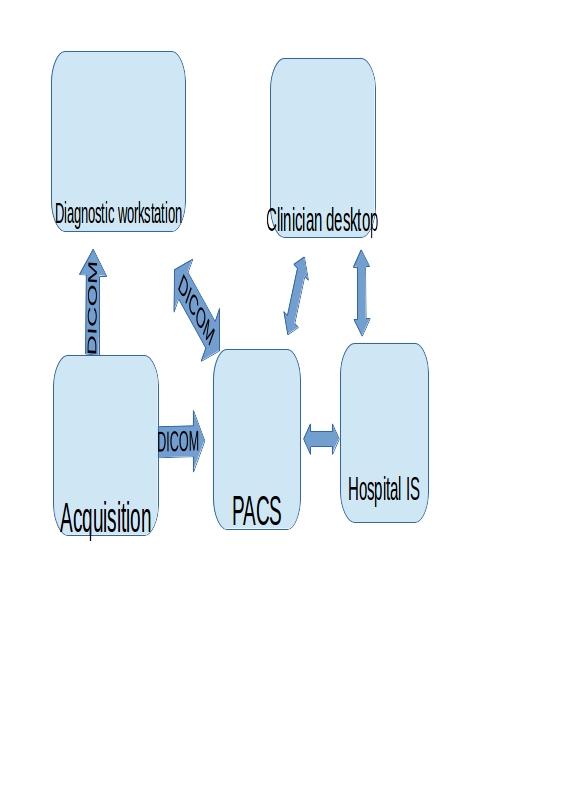
\includegraphics[width=0.8\textwidth, height=8cm]{chapter4/pacs.png}
    \caption{Typical workflow of medical image in hospital. Data acquisition is made by modalities (magnetic resonance, ultrasonography, X-ray radiography, etc.) and using DICOM format and protocol it can be directly transferred and visualized by diagnostic workstation. With metadata filled by an expert physician the image is stored in PACS. Other desktops within hospital can retrieve the image and review the report. The hospital information system may be involved in other workflows and communicate with other formats and standards (HL7,...)
    }
    \label{fig:pacs}
\end{figure}

As the data processed in hospital information systems contains sensitive information of real patients, these are protected and processing and storing is regulated by the national or international laws or agreements.
Development of telecomunication and network technologies a enabled telemedicine -- providing healthcare over remote distance. It requires to share and exchange  sensitive data of real patient among different helthcare providers and additionaly such data may be very valuable for further research. Security and encryption should be addressed and DICOM standard itself doesn't solve security issues appropriately, thus encyption during transferring the data over computer network must be ensured by other techniques.

In the Czech Republic, there exists several projects in production interconnecting different hospitals, clinics and other healthcare organization to exchange medical images. Project ePACS allows interconnecting each participant's PACS system via dedicated VPN channel to the central node and exchange of medical images are realized by routing the data flow from one VPN channel to the other\footnote{ePACS:\url{http://www.epacs.cz}, accessed January 2015}. Another approach is used in the project MEDIMED held by Masaryk University in Brno. Instead of dedicated VPN channel, they use  SSL encryption over standard TCP/IP communication and regional hospitals and healthcare providers are interconnected via the MEDIMED servers \cite{Slavicek2010}.% \cite{Javornik2011,Zatloukal2012}.
In other countries, there were tested cross-border teleradiology in projects Baltic e-health, R-Bay and others \cite{Ross2010,Saliba2012}.
These projects are focused on sharing the medical images and other knowledge and information.

Access to the wide range of medical images is needed for research of new processing and diagnostic methods, rare diseases, developing new detection algorithm etc.  DICOM records "de-identified" (identification of patient records are deleted, only date of the bird and other data are kept) or anonymized (additional information are manipulated to prevent disclosure) for research purposes to protect sensitive personal data, but keep important information for research purposes. The Globus MEDICUS project published by Erberich et al.\cite{Erberich2006,Erberich2007} is based on Globus Toolkit middleware to federate clinical and research application via a grid-computing infrastructure. Currently the project is hibernated since 2008 and no further development was published\footnote{\url{https://dev.globus.org/wiki/Incubator/MEDICUS} accessed February 2015}. Similar effort was done with a project Medical Data Manager which uses gLite grid middleware published by Duque, Montagnat et al.\cite{Duque,Montagnat2007} \footnote{\url{http://modalis.i3s.unice.fr/softwares/mdm/start} accessed February 2015} or MediGRID project published by Krefting et al.\cite{Krefting2009, Krefting2010}. Additionally to the sharing medical images, processing of images within selected use-cases supported by the grid-computing infrastructure is introduced\cite{Krefting2010}. Health-e-child project aimed to interconnect research institution and hospitals in UK, France and Italy for the purpose of grid-based healthcare platform for pediatric health-care \cite{Skaburskas2008}. Neurist project developed architecture and connects clinicians and researchers to improve research and treating of cerebral aneurysm to provide tools to analyze and interpret patient data and researcher can have access to set of aneurysm data, published by Benkner et al.\cite{Benkner2010}.
SEAGRIN research project aimed to  share knowledge mainly for educational purposes in semi-formally described semantics and such proposal and implementation was published by Kuba et al.\cite{Kuba2006}. 

Storing the sensitive medical information even de-identified or anonymised is usually restricted and this lead to an idea to store such information within trusted institution e.g. hospital and move and facilitate deployment of the grid services storing medical data to that institution. E.g. pre-installed virtual machines can contain grid-services and deployed in as a sealed grid as proposed by Kuba et al. \cite{Kuba2007a}.


%When we look to the architecture of the systems of sharing medical images the problematic part within the point-to-multipoint architecture is the central part of the systems already in production e.g. in Czech Republic (MEDIMED, ePACS). This may become single point of failure and bottleneck.

To summarize this section, digital medical image acquisition, store, exchange and processing became common in the past years and is currently using distributed computing techniques. There are several efforts to implement medical data management within grid or cloud infrastructure for research purposes and integrate them with the production infrastructures. Security is solved by authentication, authorization mechanism as well as by encrypting the data and/or de-identification or anonymization but keeping minimal information required for research purpose. A related question is  how easily the previously mentioned grid-based technologies can be integrated with current systems in hospitals or institutions. The following section describes selected methods used to integrate a pilot deployment of Globus MEDICUS with current regional system for exchanging medical images - MEDIMED.

\subsection{Methods to share medical images in grid}
\label{sec:methodsimages}

Globus toolkit belongs to the group of most used grid middleware (see section~\ref{sec:servicegrid}). The core services included in Globus Toolkit are GridFTP -- grid extension to file transfer protocol(FTP) implements strategies such as \emph{stripping data} into multiple pieces, \emph{parallel transfer of data} utilizing stripped data parts to be transfered via different channels, \emph{partial file transfer} some application may not need to acess the whole file, but a smaller portion of it. etc. \cite{Foster2006, Allcock2005}. Other core services are Replica Location Service aiming to localize data, Globus Resource Allocation Management (GRAM) provides web service and proxies to the lower level job schedulers implementation \cite{Foster2006}.

Next to core services, the domain specific services might be implemented for the purpose of application using the open grid service architecture (OGSA). Globus MEDICUS \cite{Erberich2006,Erberich2007} contains a DICOM Grid Interface Service (DGIS) and integrates the open source PixelMed\texttrademark ~Java DICOM Toolkit\footnote{\url{http://www.pixelmed.com/} accessed February 2015} into a web service communicating via DICOM protocol and on the other side it forwards the queries to underlying services within Globus toolkit. 

DGIS behaves as a gateway to a grid infrastructure. Because communication via DICOM protocol is not secured, the DGIS is recommended to be installed on the location of the PACS system or DICOM ready modality or software.
When a DICOM study is uploaded into DGIS, it is anonymized and stored and a record is made into another services Meta Catalog service which resides in the same domain or anywhere in grid accessible via Globus Toolkit.
Such anonymized database of DICOM records can be used to query via DGIS interface and to e.g. integrate with web based application showing records for research purposes, authentication and authorization can be done in this level. 
To integrate this system with existing system for sharing the medical images (e.g. the MediMed project\cite{Slavicek2010}) the special client software "RediMed console" needs to be installed next to the DGIS and configured it as a local PACS system whose records might be exchanged to other MediMed participants. 
The results of this particular deployment and integration is in section \ref{sec:resultsimages}.
%The software for processing medical images can retrieve them from DGIS via DICOM protocol. 

%To present DICOM studies The integration strategy based on shared database or files can be used to present the DICOM studies via web portal. Additionally the web portal might generate specific DICOM queries to DGIS.


%The following section will cover methods related to the integration effort.

%The section~\ref{sec:introintegration} describes several general software architectural styles and integration patterns used in further in this work. 
%The section~\ref{sec:methodsimages} describes specific methods used in the area of processing  medical images within grid infrastructure to verify the integration effort between research and hospitals systems. The section~\ref{sec:methodsvoice} describes a method to deploy existing application as a service to the distributed infrastructure.The section~\ref{sec:methodsmodels} focus on modelling methodology in order to build and maintain complex models of human physiology as the complex models seems to mainly benefit from parallel computation. And the subsection~\ref{sec:methodsmodelsestimate} follows up on the modeling methodology to describe the system for estimating model parameters. 

%as a program to start within remote session and , the interactive application allows select type of voice which will be analysed. After recording is finished, the whole recording is analyzed with FFT to obtain full spectral analysis. 

%\section{Integrating heterogenous systems}
%\label{sec:introintegration}
%
%Integrating heterogenous system into a well designed enterprise application has some issues which needs to be addressed.
%
%One of the first decision which may be hard to change in future is platform. Platform might be determined by third party platform-specific product incorporated in a workflow which cannot be changed. There exists software platforms that may run on different operating systems. E.g. Java platform is based on the idea that a program is compiled into bytecode which is then interpretted by just-in time compilers on target platform. Similar approach applies to Common Language Infrastructure (CLI) known by it's implementation .NET Framework on Microsoft Windows operating system or MONO which is implemented on Linux platforms.
%Another approach to address the issue of a platform is virtualization as mentioned already in section \ref{sec:introvirtual}.
%
%
%%\subsection{File exchange}
%Is based on the fact, that one process produces a file which is consumed by another process. This is popular in batch processing systems which needs no or only limited interactivity with user. The grid workflow management systems 
%\subsection{Message Oriented Integration}
%The processes that run concurently synchronize and exchange messages via some dedicated channel. E.g. platform depended
%
%\subsection{Service Oriented Architecture}
%\label{sec:methodssoa}
%Service oriented architecture (SOA) decouples a service contract with intention to be platform independent from it's platform-dependent implementation\cite{Erl2008}. The loosely coupled modules conforming the SOA style are realized as web service which contracts are described in Web Service Definition Language (WSDL) which defines the service interface in term of endpoint location (URL), sset of operation, binding of operation to endpoint, the format of input and output messages and binding of the messages to the operations. These are usually based on some XML dialect. Even the WSDL can be written by hand, it can be generated by a service stack framework for the concrete service implementation. 
%Next to the service implementation there are abstraction like registry and repository holding metadata of the service, so it can be dynamically discovered.
%
%\subsection{RESTful web services}
%\label{sec:methodsrest}
%The Representational State Transfer (REST) architectural style proposed by R. Fielding\cite{fielding2000chapter} is used for representing functionality as a limited  for solving demand issues of the selected tasks 
%

%The images produced by medical devices are mainly in a DICOM standard which describes the file format and communication protocol for exchange, query/retrieve image, modality and other metadata \cite{dicom2011}. The file format consist of header which involves information about the patient and the pixel data containing uncompressed or compressed bitmap of image. Some devices produces multi-frame multi-dimensional images which can be stored in one DICOM file. The DICOM standard is used to interconnect multiple medical devices, local computers and database system which is usually termed as Picture Archiving and Communitation System (PACS). 


%The particular methods used within specific biomedical domains are covered in further chapter section \ref{sec:methodsimages}, \ref{sec:methodsvoice}, \ref{sec:methodsmodels}. 

%This chapter covers general methods which might be utilized in any domain. The section~\ref{sec:introintegration} describes several general software architectural styles and integration patterns and section~\ref{sec:introvirtual} covers virtualization technology.


%The section~\ref{sec:introintegration} describes several general software architectural styles and integration patterns used in further in this work. 
%The section~\ref{sec:methodsimages} describes specific methods used in the area of processing  medical images within grid infrastructure to verify the integration effort between research and hospitals systems. The section~\ref{sec:methodsvoice} describes a method to deploy existing application as a service to the distributed infrastructure.The section~\ref{sec:methodsmodels} focus on modelling methodology in order to build and maintain complex models of human physiology as the complex models seems to mainly benefit from parallel computation. And the subsection~\ref{sec:methodsmodelsestimate} follows up on the modeling methodology to describe the system for estimating model parameters. 


%\begin{itemize}
%\item{ 
%The \emph{Service Oriented Architecture} (SOA) is high level programming model based on self contained units of functionality and metadata, so the service can be dynamically discovered and used. An important aspect is separated service implementation from it's contract or interface \cite{Erl2008} and is usually realized by web services. %More about SOA is in section \ref{sec:methodssoa}.
%}
%\item{
%The \emph{Representation State Transfer} (REST) specifies several architectural constraints that helps scalability, performance and presents functionality via fixed number of operation and uniform resource location \cite{fielding2000chapter}. %More about RESTful web services is in section \ref{sec:methodsrest}
%}
%\end{itemize}
%
%Software architecture of the distributed systems are studied and some repeating patterns are cataloged e.g. by Fowler et. al\cite{Fowler2003}. Integration patterns are discussed with focus on the ways of connecting heterogenous parts of the system as presents Hohpe et al.\cite{Hohpe2002}.

\section{Voice Science}
\label{sec:voice}
With introduction of objective data analysis and laryngoscopy methods the voice science emphasized the cooperation among  laryngologist, speech pathologist and voice teacher.
The human voice ranges from 50 Hz to something about 1000 Hz, but there are large  individual variation. For analysis of digitally recorded voice, either habitual or singing, the Discrete Fourier Transformation(DFT) is used to produce frequency and amplitude analysis of recorded input voice samples. One of the most used class algorithm to compute DFT is class of Fast Fourier Transformation with computational complexity $O(n \log(n))$ \cite{Cooley1965,Frigo2005}.
% and parallel version of the algorithms may introduce additional speedup for larger samples of analyzed data \cite{Gupta1993,Takahashi2003}. 
The result of analysis can be visualized in a voice range profile and there can be seen significant difference between untrained and trained voice as well as quantitatively seen some disorders  \cite{DeLeoLeBorgne2002,wuyts2003effects}.

Other methods to analyse vocal chords is laryngoscopy. The videostroboscopy and high speed video in laryngoscope methods produce video for analysing the real movement of vocal chords. The videokymography method introduced by Švec et al. complements the videostroboscopy and allows to visualize and analyze movement of vocal cords recorded by high speed camera on standard TV or monitor with an artificial image built from recorded sequence of selected section \cite{Svec1996,Svec2007}. 

In case of recorded sound and further analysis there is a question about how such a service can be integrated in grid-computing or cloud-computing environment to provide access to a complex application for non-technical voice specialists. Additionally, the analytical software was already developed and calibrated for selected sorts of microphones in MS Windows platform \cite{Fric2007,Fric2012}. Therefore I proposed and implemented a method that provides access to the analytical software remotely. The section \ref{sec:methodsvoice} describes how the analytical software was customized with a remote desktop protocol (RDP). Results are described in section \ref{sec:resultsvoice}. Similar approach might be used for processing the video recordings from laryngoscope, however, the practical limits are discussed in section \ref{sec:conclusion}. 

\subsection{Methods for remote analysis of human voice}
\label{sec:methodsvoice}
%One method to provide access to specialized service is via remote access protocols. Secure Shell (SSH) is used to establish secure channel via unsecured network (e.g. the Internet) from SSH client to SSH server providing e.g. remote command-line, remote command execution etc. It is one of the basic method to access the grid infrastructure and submit computational jobs. 
%Another method is to have a web portal and this web portal based on user's input executes command-line batch scripts over SSH, or it can utilize web services to submit computational job.
Terminal access to some remote computational capabilities, e.g. remote command-line or remote execution is another integration strategy to some remote infrastructure. Secure Shell (SSH) is used to establish secure channel via unsecured network (e.g. the Internet) from SSH client to SSH server and it is basic method to access grid-computing infrastructure. 

Remote Desktop Protocol(RDP) is a proprietary protocol for desktop sharing developed primarly in Microsoft Windows platform, however, today clients and servers exists for several other platforms. Next to remote command-line, remote execution it allows to access remote graphical desktop environment. %VNC is sharing protocol to access remote graphical desktop environment\cite{Richardson1998}. 
The software for parameterized Voice Range Profile (ParVRP) and Voice Range Profile in Real time (RealVoiceLab) was already developed and calibrated for selected sorts of microphones in MS Windows platform by Fric et al.\cite{Fric2007,Fric2012}. The implementation is done in MATLAB environment utilizing Signal Processing Toolbox\footnote{\url{http://www.mathworks.com/products/signal/} accessed February 2015}and compiled with MATLAB Compiler and distributed as an executable.

Instead of migrating the application into some compatible platform for grid-middleware, a virtual machine was introduced and access to the software is provided via RDP protocol. RDP itself contains redirection of several services, e.g. sound recording or drive access. Because the default sound recording redirection introduces some sound degradation without control, I proposed, implemented and integrated the custom RDP plugin with the ParVRP and RealVoiceLab software to redirect the sound recording without loss of information. Technical details are in Appendix~\ref{app:remote}. 

The computation of frequencies and amplitude from the recorded samples utilizes Fast Fourier Transformation which has time complexity $O(n\log(n))$ and current implementation are fast on any even modile devices. The benefit from deploying such application in distributed infrastructure is immediate access to updated software and a collection of anonymized records of voice samples with analyzed results for further research and education purposes.

This type of application can be packaged as virtual machine template and configured within different types of cloud infrastructures and together with a script or web portal the on-demand deployment can be automated. The client part (RDP client) needs to connect to the appropriate instance. The results of such deployment are discussed in section~\ref{sec:resultsvoice}.

\section{Computational physiology}
\label{sec:models}
A mathematical formalization of the fundamental knowledge and relation among biological system - mathematical model - is used as a base abstraction to utilize current discoveries of the genomics and proteomics and formalize the knowledge and construct a "Physiome Model". Model by it's definition is simplification of the complex reality.

Constructing the models and integrating them into complex entity which can be used for further purposes is schematically illustrated in fig. \ref{fig:modeling}. The measurements are done in laboratories or in hospitals. Lumped parameter models are usually represented as ordinary differential equations and differential algebraic equations and characterize the reality as topology of discrete elements. The imaging methods for processing and analysis (section \ref{sec:imaging}) are used to construct 3D models from segmentation and generating of mesh representation connected to physical principles. 
\begin{figure}[ht]
    \centering
    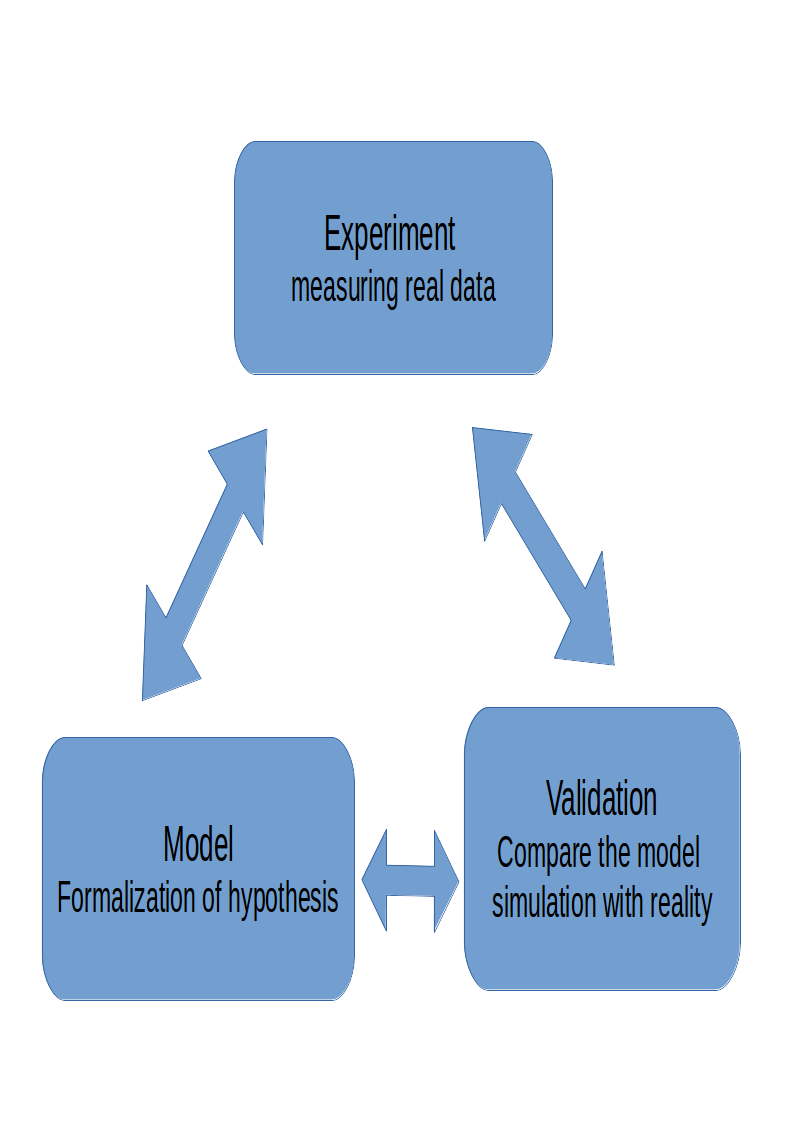
\includegraphics[width=0.5\textwidth, height=5cm]{chapter6/modeling.png}
    \caption{Schematic illustration of scientific process. The experiments produces data which are interpreted and hypothese is formalized as a model. Validation compares the model simulation with experiment, if model satisfies the criteria - is in agreement with real experiments, then the validated model can be used for other purposes.  %\bibentry{EGICompendium2013} \bibentry{egi2014}.
    }
    \label{fig:modeling}
\end{figure}

Application of the mathematical modelling techniques towards the biomedical research is sometimes called as systems biology approach combining the reductionism and integration as denoted by Kohl et al.\cite{Kohl2010}. Application towards the clinical praxis include the quantification of the diagnostic index or treatment strategy and it is a goal to develop tools, database models and methods of several Physiome projects, e.g. VPH-Physiome project presented by Hunter et al.\cite{Hunter2009}.

One of the earliest complex and integrative modelling effort was a model of circulation and it's regulation published by Guyton et al. in 1972 \cite{Guyton1972} which via derivative and technological upgrade continues as "Human Model" or "HumMod" introduced by Hester et al. \cite{Hester2011systems,hester2011} with a focus on integration effort. Different approach of modelling human physiology is a database of smaller models focusing on some particular physiological phenomenon. E.g. the NSR Physiome project introduces  JSIM\footnote{JSIM: \url{http://www.physiome.org/jsim/} accessed January 2015} Java based simulation system to support modeling in  physiology. Repository of several hundred of models were published using this system \cite{Butterworth2014}. The similar effort is done by IUPS Physiome project and repository of models are  based on XML standard languages CellML and FieldML \cite{Hunter2004,Yu2011}. The Systems Biology Markup Language (SBML) is used for modeling biological system at the level of biochemical reaction and regulatory network and another database collects several hundreds of curated and non-curated models \cite{Hucka2004,LeNovere2006}.

JSIM, CellML, SBML or HumMod are domain specific languages and the tools able to work with them are primarily developed within physiological or systems biological communities. Other authors use commercial or industry standard tools for mathematical modelling and computing. E.g. Kofranek et al. describes Guyton's 1972 model in MATLAB\textsuperscript{\textregistered} Simulink \cite{Kofranek2010} and the derivative HumMod in acausal object-oriented Modelica language \cite{Kofranek2011hummod,kofranek2013hummod}. Fernandez et al. describes models of cardiovascular pulsatile system using MATLAB Simscape  \cite{FernandezDeCanete2013} and recently in Modelica  \cite{FernandezdeCanete2014}.

Thus there is an open debate whether in-house domain specific language and tools like JSIM, CellML and FieldML,SBML or HumMod reached it's capabilities for representing complex models. Only the HumMod reached the integrative approach building the complex integrative model of human physiology using lumped parameter approach. I contributed to the idea of key features which involves acausal modeling technique and object orientation which keeps the complex model structure decomposed into understandable and maintainable parts and allows to cover complexity of models like HumMod. 

The methods and examples of modeling cardiovascular system are described in the next section \ref{sec:methodsmodels}. The methods of estimating parameters of complex models are described in section \ref{sec:methodsestimation} and particular results are described in section \ref{sec:resultsestimation}.

%\label{sec:results}
\subsection{Modeling methodology}
\label{sec:methodsmodels}
%For building complex models it seems that acausal (or declarative) modeling technique is key feature as it allows to express the variables declaratively, acausal modeling tool (e.g. Modelica or MATLAB\textsuperscript{\textregistered}  SIMSCAPE\texttrademark) figures out which are the dependent and independent variables upon compilation\cite{fritzson2002}. This allows building complex systems of equation from composed components and the model diagrams still captures the essence of the modeled reality much better and the simulation models are much more legible and thus also less prone to mistakes\cite{Kofranek2008,FernandezDeCanete2013}. 

The methodology of formalizing mathematical models is influenced by the abilities of underlying modeling language used. 
The Modelica language is an object-oriented, equation based and acausal modeling language standardized by Modelica association\footnote{\url{http://www.modelica.org} accessed February 2015}.

%\emph{Object orientation} means that the definition of model is class as in object oriented programming, instance of the model is object,  each instance can share type and differ in parameters and the place where it is used, inheritance and some sort of polymorphism is possible.
%\emph{Equation based} means that the equation is not statement, thus the relation among variables can be expressed in any form and Modelica tool will decide which one is input and output upon compilation. %E.g. from the equation $q = \frac{dV}{dt}$ the process of computation can lead to $ q:= der(V)$ or $ V := \int{q}dt$ based on whether the $V$ or $q$ is known from the context.
%\emph{Acausal} connector is special purpose class to define variables of the model shared with other models or classes. Connecting two or more components via acausal connector will generate analogy of Kirchhoff's law: equality of all "non-flow" variables in connected connectors \begin{equation}p_1=p_2=\ldots =p_n\label{eq:kirchhoff1}\end{equation}
%and zero sum of all "flow" variables \begin{equation}\sum_{i=1}^n q_i=0\label{eq:kirchhoff2}\end{equation}
%
%To model e.g. cardiovascular system (CVS) we can decompose it to abstract component expressing hydraulic elasticity and hydraulic resistance. Connector \emph{HydraulicPort} with "flow" variable $q$ and non-flow variable pressure $p$ is presented in Modelica source code:
%\begin{lstlisting}[language=modelica]
%connector HydraulicPort
%  flow Real q;
%  Real p;
%end HydraulicPort;
%\end{lstlisting}
%Model of hydraulic resistor(conductor) with parameter $G$ denoting conductance and two hydraulic ports express the equations:
%\begin{equation}
%q_{in}.q = -q_{out}.q \label{eq:conductor1}
%\end{equation} 
%\begin{equation}
% q_{in}.q = G \times (q_{in}.p-q_{out}.p) \label{eq:conductor2}
%\end{equation}
%Model of hydraulic elastance with parameters $V_0$ as unstressed volume $p_0$ external pressure and $C$ compliance(reciprocal value of elastance) with state variable $V$ volume express these equation:
%\begin{equation} \label{eq:elastic1}p-p_0 = \left\{   
%  \begin{array}{l l} 0 & \quad \text{if } V \text{\textless} V_0 \\ 
%    \frac{V-V_0}{C} & \quad \text{otherwise}
%  \end{array} \right.\end{equation} 
%\begin{equation}\label{eq:elastic2}\frac{{\rm d}V}{{\rm d}t} =  q\end{equation} 
%Both models can be written in Modelica as:
%\begin{lstlisting}[language=modelica,multicols=2]
%model HydraulicConductor
%  parameter Real G;
%  HydraulicPort qin;
%  HydraulicPort qout;
%equation 
%  qin.q= -qout.q; // eq.(3.3)
%  qin.q = G*(qin.p-qout.p); // eq.(3.4)
%end HydraulicConductor;
%
%
%
%model HydraulicElastance
%    Real V;
%    parameter Real V0;
%    parameter Real p0;
%    parameter Real C;
%    HydraulicPort qin;
%equation 
%   // eq.(3.5)
%  qin.p-p0 = if (V<V0) then 0 else (V-V0)/C;
%  der(V) = qin.q; // eq.(3.6)
%end HydraulicElastance;
%\end{lstlisting}
%
%This can be used to model two ideal baloons with liquid  interconnected via a tube characterized by some resistance. The acausal connectors \emph{qin} and \emph{qout} are connected via the \emph{connect()} statement in the following listing:
%\begin{lstlisting}[language=modelica]
%model twoballons
%  HydraulicConductor systemicResistance;
%  HydraulicElastance arteries;
%  HydraulicElastance veins;
%equation 
%  connect(arteries.qin, systemicResistance.qin);
%  connect(systemicResistance.qout, veins.qin);
%end twoballons;
%\end{lstlisting}
%
%The concrete instances may differ e.g. in a way what is known of the system, either by external measurement, or by some superior model. The \emph{ballsVolume} is initialized with initial volume of first balloon \emph{V(start) = 5000}. But the model \emph{ballsFlowPressure} is initialized with initial pressure generated by the baloon \emph{p(start) = 2980.67}.
%\begin{lstlisting}[language=modelica,multicols=2]
%model ballsVolume
%  extends twoballons(
%    arteries(
%      V(start=5000),
%      V0=529,
%      p0=0,
%      C=1.5),
%    systemicResistance(G=1),
%    veins(
%      V0=2845,
%      p0=0,
%      C=200));
%end ballsVolume;
%model ballsPressure
%  extends twoballons(arteries(
%      V0=529,
%      p0=0,
%      C=1.5,
%      qin(p(start=2980.67, fixed=true))),
%    systemicResistance(G=1),
%    veins(
%      V0=2845,
%      p0=0,
%      C=200));
%end ballsFlowPressure;
%\end{lstlisting}
%Based on an concrete instance of the model with specific initial condition, the Modelica tool will decide what will be dependent and  what independent variables and computation flow based on the above rules and equation is generated as in following statements with assigning symbol (\emph{:=}).
%\begin{lstlisting}[language=modelica,multicols=2]
%// Translated M. model generated by Dymola  
%//  ballsVolume
%
%
%
%// Dynamics Section
%  systemicResistance.qout.p := veins.p0+
%    (if veins.V < veins.V0 then 0 
%    else (veins.V-veins.V0)/veins.C);
%  systemicResistance.qin.p := arteries.p0+
%    (if arteries.V < arteries.V0 then 0
%    else (arteries.V-arteries.V0)/arteries.C);
%  der(arteries.V) := systemicResistance.G*
%    (systemicResistance.qout.p-
%      systemicResistance.qin.p);
%  der(veins.V) :=  -der(arteries.V);
%
%
%
%// Translated M. model generated by Dymola 
%// ballsPressure
%// Initial Section
%...
%// Dynamics Section
%  systemicResistance.qout.p := veins.p0+
%    (if veins.V < veins.V0 then 0 
%    else (veins.V-veins.V0)/veins.C);
%  arteries.qin.p := arteries.p0+
%    (if arteries.V < arteries.V0 then 0 
%    else (arteries.V-arteries.V0)/arteries.C);
%  arteries.qin.q := systemicResistance.G*
%    (systemicResistance.qout.p-
%      arteries.qin.p);
%  der(veins.V) :=  -arteries.qin.q;
%  der(arteries.V) := arteries.qin.q;
%\end{lstlisting}
%

%
%Empirically derived function of flow rate per time going out from the heart:
%\begin{equation} \label{eq:heart} q = \left\{   
%  \begin{array}{l l} 0 & \quad \text{otherwise} \\ 
%    \sin \left( 
%    \frac{t_c-T_{D1} }{ T_{D2} -T_{D1} } * \pi \right) * Q_{peak} 
%    & \quad \text{if } t_c \in (T_{D1}..T_{D2})
%  \end{array} \right.\end{equation} 
%\begin{equation}\label{eq:flowrate2}\frac{{\rm d}V}{{\rm d}t} =  q\end{equation} 
%
%\begin{lstlisting}[language=modelica]
%model HeartFlow
%  HydraulicPort qout;
%  discrete Real T0, HP=0.8;
%  Boolean b(start = false);
%  parameter Real TD1 = 0.07, TD2=0.39, QP = 0.000424;
%  Real tc "relative time in cardiac cycle";
%equation
%  b = time - pre(T0) >= pre(HP) "true if new cardiac cycle begins";
%  when {initial(), b} then
%    T0 = time "set begining of cardiac cycle";
%  end when;
%  tc = time - T0 "relative time in carciac cycle";
%  qout.q=if tc>TD1 and tc<TD2 then sin((tc-TD1)/(TD2-TD1)*Modelica.Constants.pi)*QP else 0;
%end HeartFlow;
%\end{lstlisting}

The paper \cite{Kulhanek2014Modeling} \emph{Modelling of Short-term Mechanism of arterial pressure in the cardiovascular system: Object-oriented and acausal approach} in Appendix~\ref{app:modeling} published disputation about causal and acausal approach in using Modelica for modeling pulsatile cardiovascular (CVS) system. 

The paper \cite{Kulhanek2014mefanet} \emph{Simple Models of the Cardiovascular System for Educational and Research Purposes} in Appendix~\ref{app:simplemodelsd} published detailed methodology of modeling pulsatile CVS in Modelica. 

Common guide to the Modelica language and it's capabilities are in the book of Fritzson \cite{fritzson2002} or in the on-line book by M.Tiller \cite{Tiller2014}.


\subsection{Identification of physiological systems}
\label{sec:estimation}

%\subsection{Identification of physiological systems}
%Model verification (whether simulation of the model shows desired behavior) and model validation (whether model simulation agrees with new observation of real system) are important steps in system analysis and model construction. 
Usually some knowledge of the system - the structure is available and unknown coefficients (parameters) remain unknown. Once the model is formalized and constructed, further problem is to estimate the model parameters so that the model reproduces real world system. This procedure is sometimes called system identification and the objective of parameter estimation is usually to minimize the following function (to find least squares of the differences between predicted and measured values):
\begin{equation} \label{eq:parameter} 
f( \vec{p} ) = \sum_{i=1}^{n} ( M(t_{i},\vec{p} ) - d(t_{i}) )^2 \to min  
\end{equation} 
where $\vec{p}$ is vector of values of parameters, $M(t_{i},\vec{p})$ is model simulated at time $t_{i} $ with the given parameter values $\vec{p}$ and $d(t_{i})$ is the measured experimental value at time $t_{i}$. 
In general mathematical models of biological systems are in most cases non-linear and can be non-differentiable thus local optimization methods . Algorithmically, this problem was shown to belonging to the \emph{NP-complete} problems \cite{Hofmann2005} thus the best known exact algorithm is based on brute force search - e.g. trying all possible values of parameters and simulate the model with them and find minimum of the objective function \ref{eq:parameter}.
Further reading about parameter estimation and system identification can be found in book edited by Eykhoff \cite{Eykhoff1981} or book of Khoo \cite[p.~159]{khoo2000}.

 , therefore global optimization methods should be used and are based on some heuristic to reduce the number of simulation. The evolution strategies were identified as robust with potential to utilize parallel computing as shawn by Moles at al.\cite{Moles2003}

%However, exact solution may not be needed because the models itself are by definition approximation of real system, and the input data are measured with some degree of error. 
After the parameter estimation a further problems arise with structural identifiability and analysis of sensitivity to the estimated parameter values\cite[p.~176]{khoo2000}. 

Parameter estimation and further analysis methods are part of specialized mathematical software. E.g. Pruet et al. used Metropolis algorithm to produce a distribution of parameters to calibrate the model of human cardiovascular physiology, which were further tested against predictive ability of circulatory failure and statistical methods performed in the software Wolfram \textit{Mathematica} \cite{Pruett2013}. The iterative improvement method in the software MATLAB Simulink\textregistered ~was used in estimating 2 parameters of simple cardiovascular model by Takahashi et al. \cite{Takahashi2013}. Several methods were compared in estimating multiple parameters of cardiovascular system in MATLAB Simulink\textregistered ~by Abbass et al. \cite{Abbass2012}.

Maffioletti et al. published GC3Pie framework utilizing evolutionary algorithms and introduced workflow to identify parameters of models for economical predictions using grid computing \cite{maffioletti2012computational}. Humphrey et al. calibrated hydrology models utilizing commercial Windows Azure cloud computing infrastructure with a significant speedup on the modified dynamically dimensioned search algorithm\cite{Humphrey2012,Tolson2007}. 

%Selected methods to estimate parameters are introduced in section \ref{sec:methodsmodels}. 

%As already identified also by other authors of some calibrating systems, the parameter estimation is used sporadically, however, with high demand of computational task in temporal time. Thus, I proposed and designed the system which can distribute the simulation task into grid-computing and cloud-computing infrastructure and the computational capacity can be provisioned on-demand. % this brings significant speedup for parameter estimation of complex model but limited speedup on simple models. 


\subsection{Methods for Parameter Estimation}
\label{sec:methodsestimation}

\begin{figure}[htb]
    \centering
    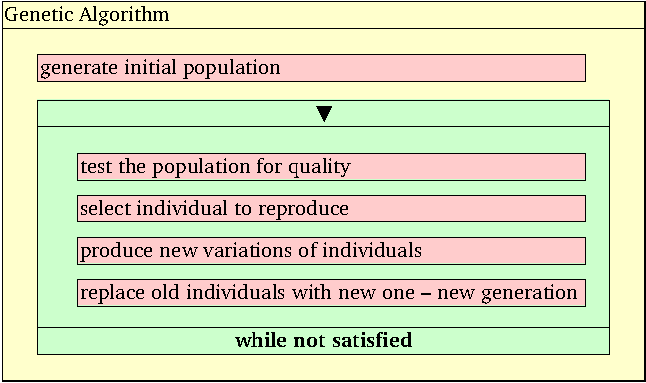
\includegraphics[page=1]{chapter3/GA-kopenogram-crop.pdf}    
%    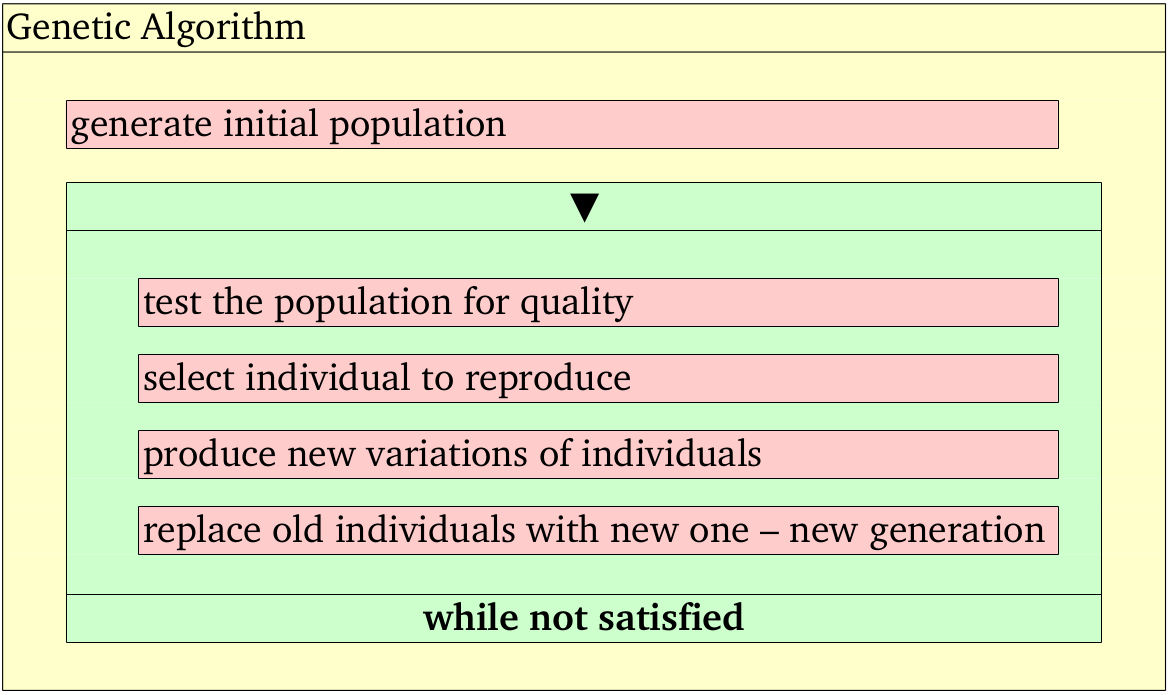
\includegraphics[width=0.5\textwidth]{chapter6/GA-kopenogram.png}
    \caption{Kopenogram of genetic algorithm. 
    }
    \label{fig:GA-kopenogram}
\end{figure}
\begin{figure}[htb]
    \centering
    \includegraphics[page=2]{chapter3/GA-kopenogram-crop.pdf}    
%    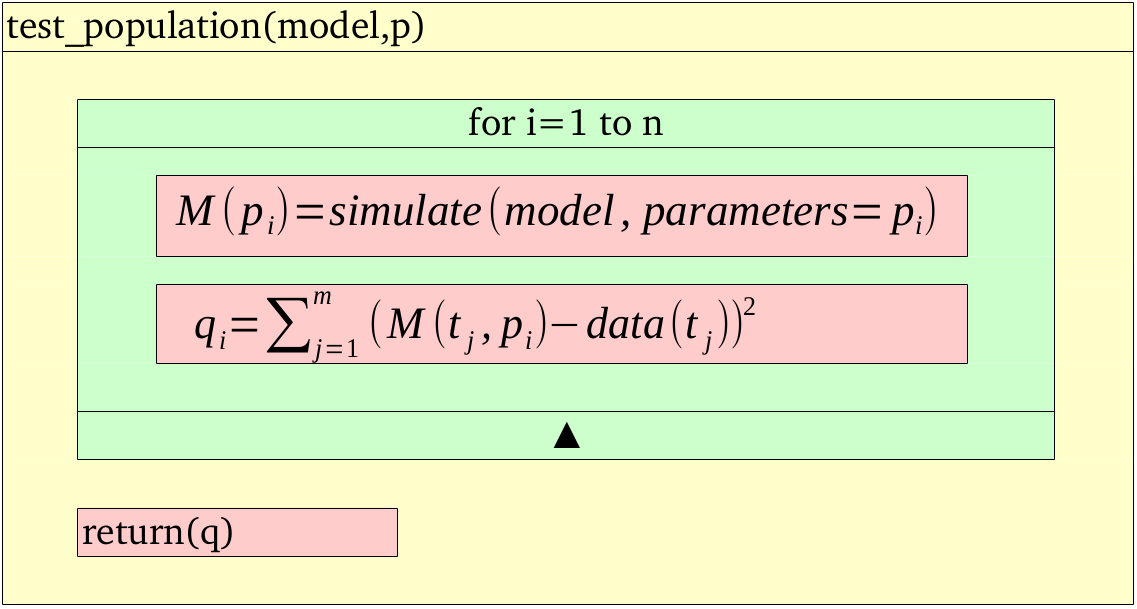
\includegraphics[width=0.5\textwidth]{chapter6/GA-kopenogram2.png}
    \caption{Kopenogram of genetic algorithm and specific test of the population for quality in case of parameter estimation. Model is simulated according to individual $i$ with parameters $p_i$ and the quality $q_i$ is counted per the objective function \ref{eq:parameter}.
    }
    \label{fig:GA-kopenogram2}
\end{figure}
Evolutionary algorithms can be used as heuristic strategy for finding global minimum or maximum and it can be used to estimate the parameters of the model. Genetic algorithm a type of evolutionary algorithm which encodes individuals as binary string was introduced e.g. by Holland\cite{Holland1975} and the algorithm steps are schematically presented in figure \ref{fig:GA-kopenogram}.

The iteration within the loop "$\blacktriangledown \ldots$ \emph{while not satisfied}" depends on previous iteration, thus it cannot be parallelized.
The step \emph{test the population for quality} has algorithmical structure in fig.\ref{fig:GA-kopenogram2} for parameter estimation tasks. Each iteration in the loop "\emph{for i=1 to n}" is independent and a therefore loop parallelism (section \ref{sec:parallelprogramming}) can be utilized and implemented here.

%The Amdahl's law in equation \ref{eq:amdahl} can be used to estimate  the theoretical speedup limitation for the specific model and potential gain for identifying different types of models can be stated. We assume that the simulation of the model with any parameters will take the same time, even this is not generally true as the non-linear models and numerical methods may cause different steps to be performed for different parameter values. 

%The specific fraction $\alpha$ for the model determines the level of scalability of the model within the parallelized system. For the complex models the $\alpha$ will decrease. The specific estimates of the fraction $\alpha$ and it's influence on the scalability and results are presented in section \ref{sec:resultsestimation}.

\subsubsection{Architecture of system for parameter estimation}
\begin{figure}[hbt]
    \centering
     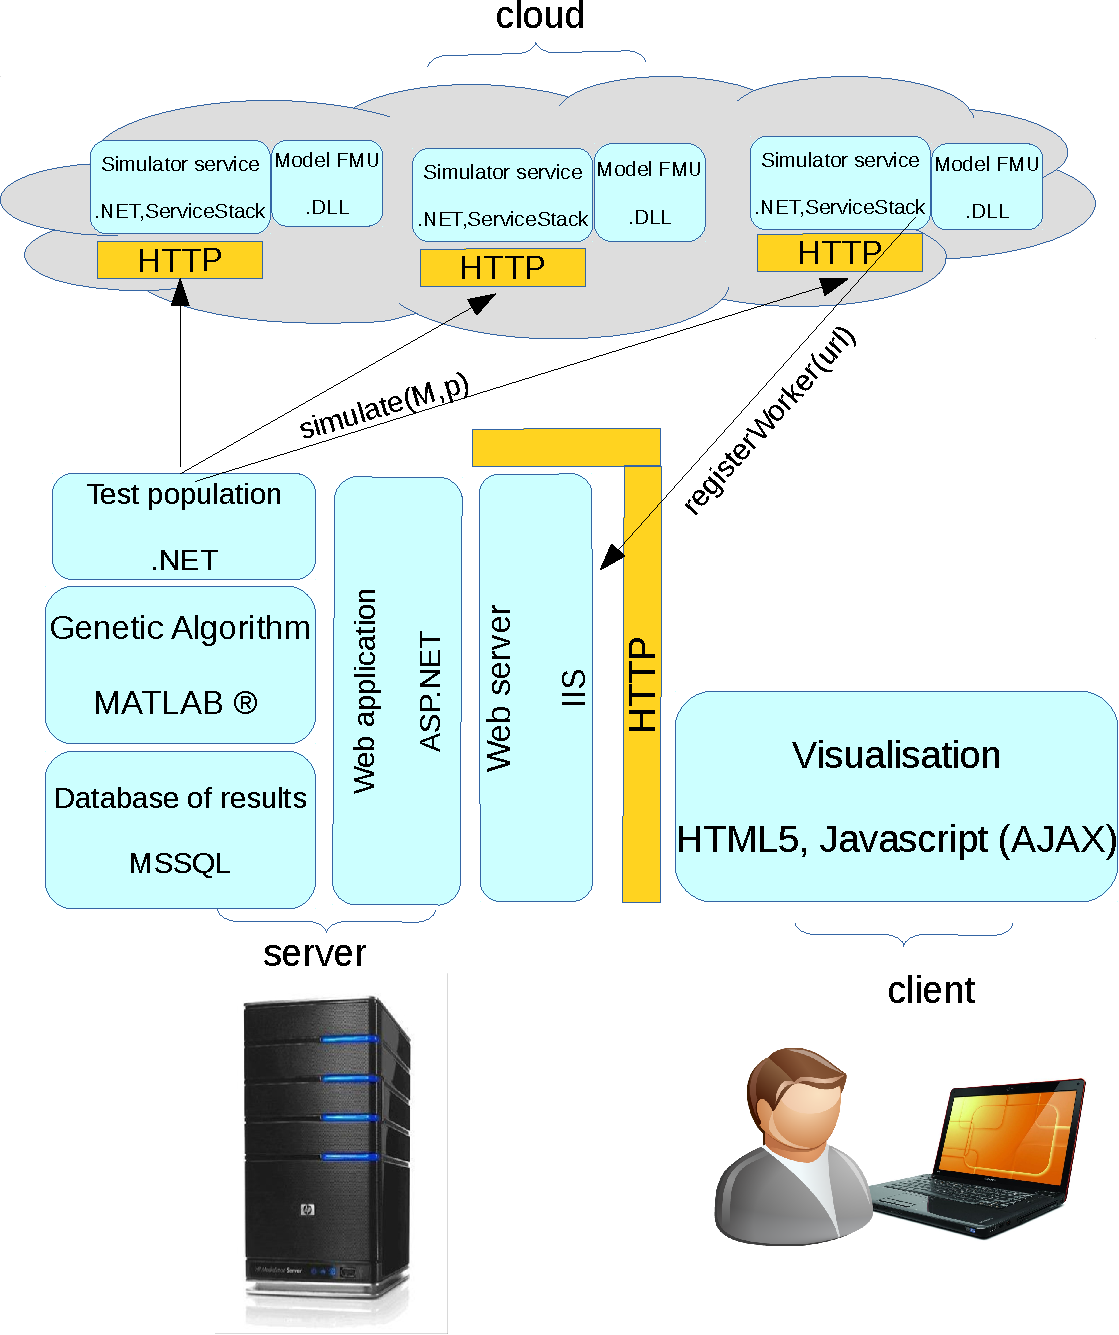
\includegraphics[page=1,width=0.75\textwidth]{chapter3/architekturaestimation-crop.pdf}  
    \caption{Architecture of the system employing genetic algorithm and distributing the \emph{simulate} task into cloud computing environment.}
    \label{fig:architectureestimation}
\end{figure}
Proposed architecture of the system for parameter estimation (fig. \ref{fig:architectureestimation}) was influenced by the need of some interactivity and overall accessibility for users which is fulfilled by the web UI. The key part of the system in opposite side is a model exported into a binary platform dependent library. 
The specific model of a studied system implemented in Modelica is exported into standard Functional Mockup Unit(FMU) with is standardized XML metadata packaged together with  binary library .DLL (or .SO) following standardized API \cite{Blochwitza}\footnote{\url{https://www.fmi-standard.org/} accessed February 2015}. In the time of writing the thesis the most stable Modelica tool export was Dymola\footnote{\url{http://www.dynasim.se} - Dymola tool, accessed March 2015} export to FMU for MS Windows platform. 

The parallelization is implemented using threads in \emph{test\_population} method which within a loop follows fork/join pattern -- the created threads simultaneously asks for simulation results with a parameter set and main process waits until all results are returned to compute full vector of quality evaluation $q$.

Packaged with .NET ServiceStack framework\footnote{\url{https://servicestack.net/} accessed February 2015} it exposes a simulation functionality as a RESTful web service which can be accessed and orchestrated by the \emph{test\_population} algorithm. The implementation of genetic algorithm is reused from MATLAB \texttrademark and with a database of results in a SQL database is integrated with ASP.NET web application presenting a web user interface and functionality to a user.
The result of applying the methods and deploying the designed system in local cluster and cloud computing infrastructure is described in section \ref{sec:resultsestimation}.

\subsection{Parameter Sweep}
\label{sec:sensitivity}
\begin{figure}[hbt]
    \centering
     \includegraphics[page=4]{chapter3/GA-kopenogram-crop.pdf}    
%    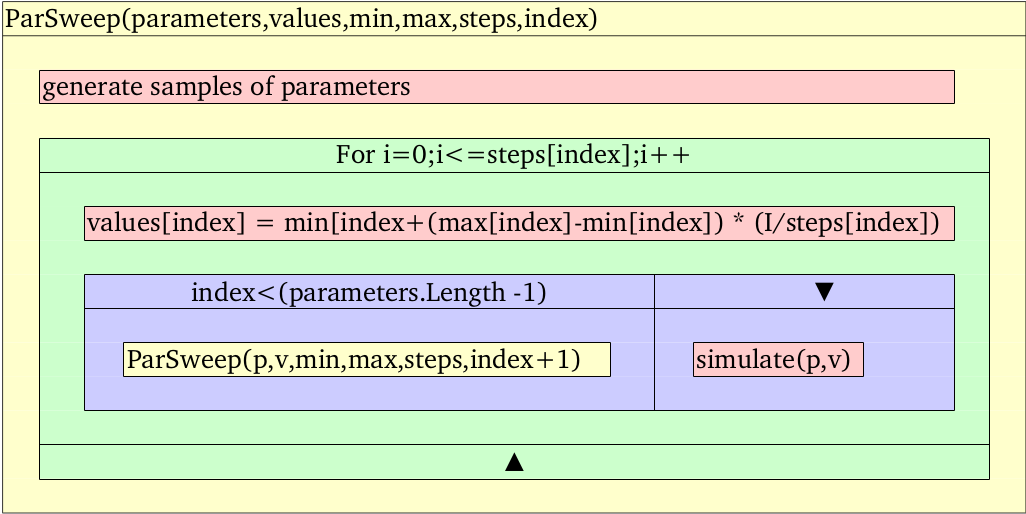
\includegraphics[width=1\textwidth]{chapter3/paramsweepkop.png}
    \caption{Kopenogram of recursive parameter sweep algorithm. $p$,$v$,$min$,$max$ and $steps$ are arrays with the same dimension holding parameter name, value, starting and stoping value and number of steps which needs to be performed between starting and stopping value per each $index$.    
    }
    \label{fig:paramsweep}
\end{figure}

Parameter sweep (PS) is one of the techniques used for sensitivity and uncertainty analysis which is based on changing selected parameters and simulating whole model and quantifying the change on model behavior with different parameters. Uncertainty and sensitivity analysis tries to determine how a change of the value of parameter will contribute to the model output and how the estimation of parameter values are robust to errors of measurement of the real data. Various methods to do uncertainty and sensitivity analysis can be found e.g. in a reviews by Helton et al. \cite{Helton2006} or a books by Saltelli et al.\cite{Saltelli2004,Saltelli2008}. 

Recursive algorithm of parameter sweep for exploring parameter space (in fig.\ref{fig:paramsweep}) generates tremendous number of simulation. Presuming that \emph{simulate} operation takes constant time for any parameters (which is not true in general) the time complexity of PS is $O(\prod_{i=1}^{n}) \text{steps}_i) \approx  O(k^n)$ where $k=\max_{i=1}^n(\text{steps}_i)$ and $n$ is number of parameters to be swept. E.g. for 1000 values for each parameter: $O(1000^n)$. The large number of distinct simulation can take tremendous time on single computer. However, in contrast to parameter estimation, each of the simulation is independent and PS algorithm is determined as embarrassingly parallel and is implemented in many grid-computing projects and workflows e.g. P-Grade portal as published by Kacsuk et al.\cite{Kacsuk2011}.

To perform parameter sweep algorithm on the models of human physiology in Modelica language an export from the Modelica is needed. The FMU standard supported by many tools exports FMU as 

a BOINC platform\cite{Anderson2004}\footnote{\url{http://boinc.berkeley.edu/} accessed February 2015} is customized following the task parallelism and master/worker programming model (reffered in section \ref{sec:parallelprogramming}). The Modelica model exported as FMU for Windows platform is integrated with BOINC wrapper and as a whole it is integrated into BOINC platform deployed on a server as seen in fig. \ref{fig:paramsweeparch}. 

\begin{figure}[htb]
    \centering
     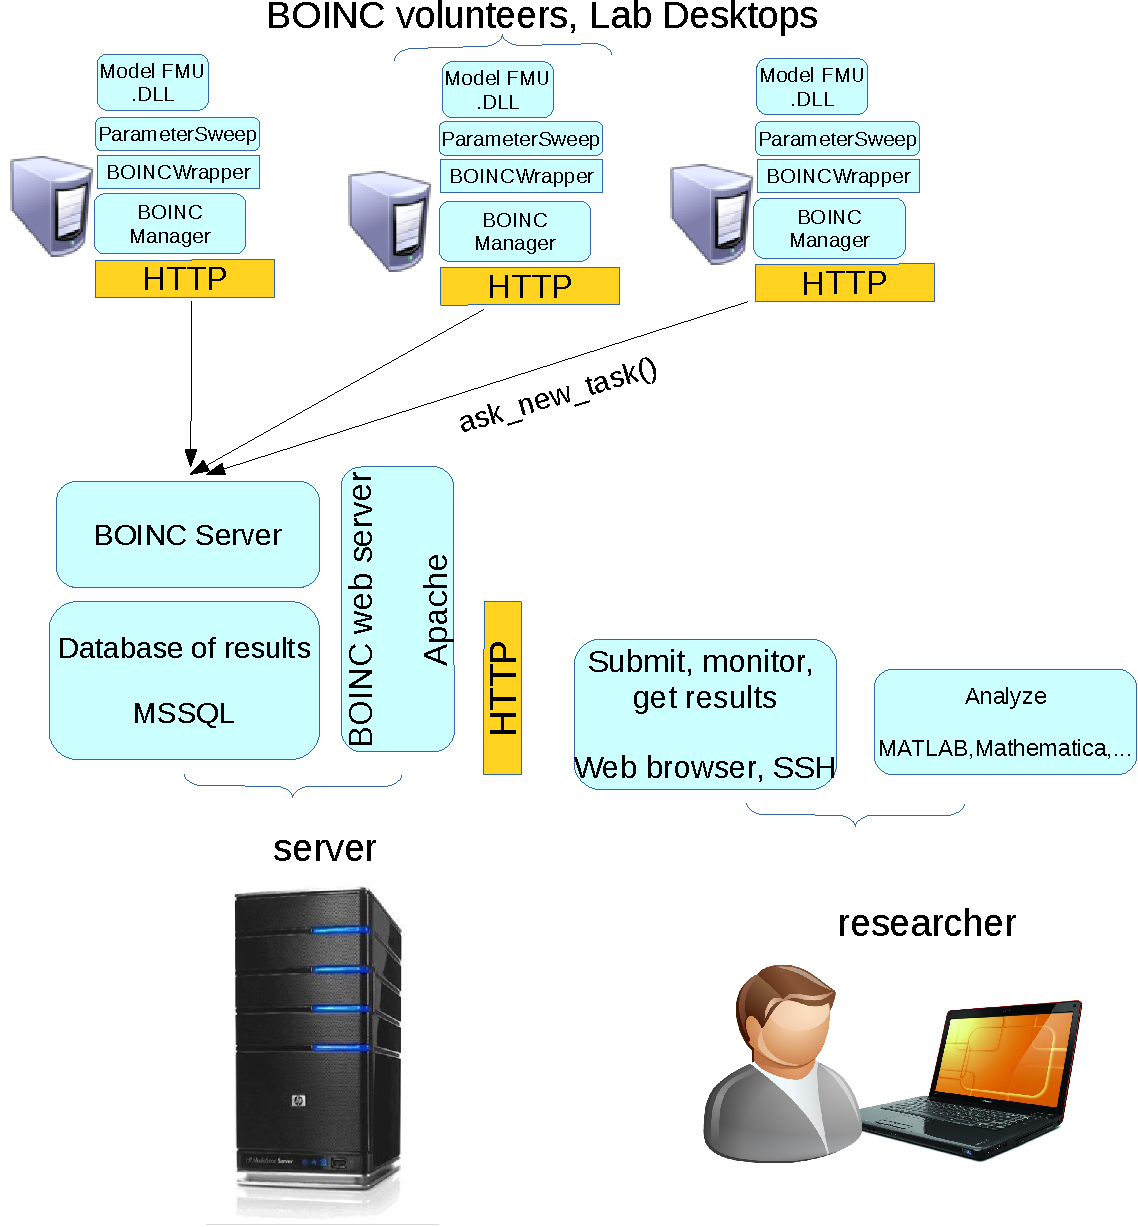
\includegraphics[page=1,width=0.75\textwidth]{chapter3/architekturaparamsweep-crop.pdf}    
%    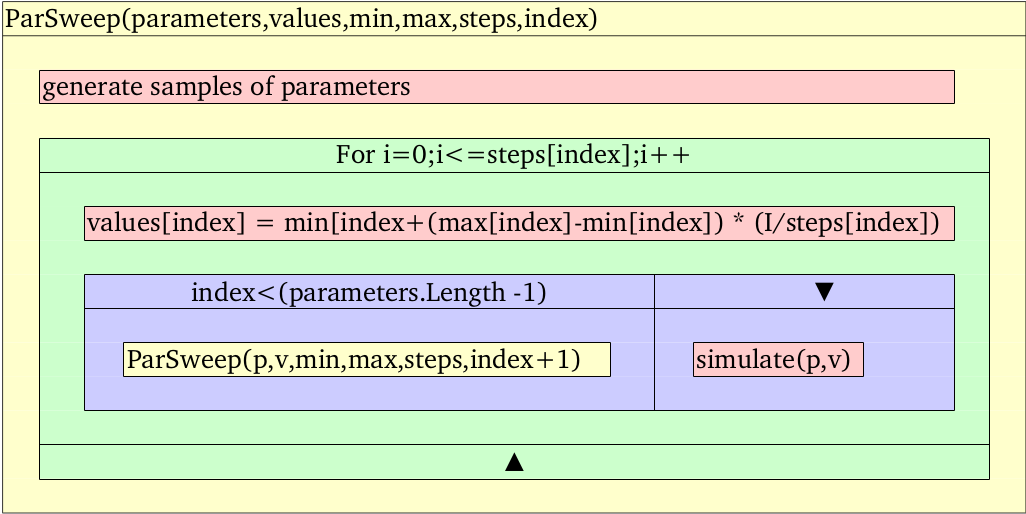
\includegraphics[width=1\textwidth]{chapter3/paramsweepkop.png}
    \caption{Architecture of parameter sweep application. The whole parameter space is divided into smaller spaces which are resolved by the BOINC workers}
    \label{fig:paramsweeparch}
\end{figure}

The results are described in section \ref{sec:resultsestimation}.

%The paper \cite{Kulhanek2011} \emph{From Educational Models Towards Identification of Physiological Systems} in Appendix~\ref{app:fromeducational} describes desktop grid system BOINC and deployment for parameter estimation mentioned in previous chapter. However, per the high latency of BOINC solution, the of the specific Modelica model exported into Windows executable into BOINC client. 
 %methods
%\chapter{Sharing medical images}
\label{sec:imaging}
%\label{sec:medicalapp}
This chapter introduces acquiring, storing and sharing digital medical images and related metadata within hospital or healthcare provider and among them and research institution.

%are covered in section \ref{sec:introimages}. Overview of analysis of speech and voice and it's relation to voice science is in section \ref{sec:introvoice}. Overview of models and simulation of human physiology and it's relation to systems biology is briefly covered in section \ref{sec:intromodels}.


%The computing in biomedicine can be divided into research and clinical application. %Translational science aims to "translate" findings from research to better health care including diagnostic tools, procedures, drugs, etc.

%In case of research use-cases, processing medical information helps to make more precise current theories or support formulating new one. In case of clinical use cases, processing medical information helps to analyse and interpret the information, predicting future trends and support decision on some intervention.

%\footnote{Motivation of using distributed computing technologies is to share physical data, among multiple organizations, where there is no need or other barriers to store all data centrally, e.g. for legal or capacity limitation. A lot of medical information within biomedical research came from real patient and such information are protected by some regulation and processing of them is regulated and controlled by the country laws or international agreements. Thus there must be considered ethical as well as legal issues how to deal with such information. Sharing and processing of medical images are covered in section \ref{sec:introimages}. Providing access to services with high values is another motivation of using distributed computing technologies. E.g. basic and advanced analysis of biological signals, especially of voice is described in section \ref{sec:introvoice}.}


Digital medical images involves the image acquisition, preprocessing, storing and searching.
Clinicians use patient image mainly for visualization and diagnostic purposes. Computer assisted methods facilitate the diagnostic process and involves image enhancement (to reduce image noise and increases the contrast), image segmentation (to separate different types of structures from background and from each other), quantification methods (to determines the structure shape, size, volume), registration methods (to process and join multiple different images into one).
Comprehensive concepts and digital techniques are presented e.g. in book edited by I.N.Bankman\cite{Bankman2000}.

Acquisition of the medical image is covered with different modalities (different types of equipment and sensors) by radiologists or other specialists. DICOM\footnote{DICOM: \url{http://dicom.nema.org/} accessed January 2015} format and standard becomes most popular to exchange medical images electronically and picture archiving communication systems (PACS) are currently parts of information systems in hospitals.

\begin{figure}[ht]
    \centering
    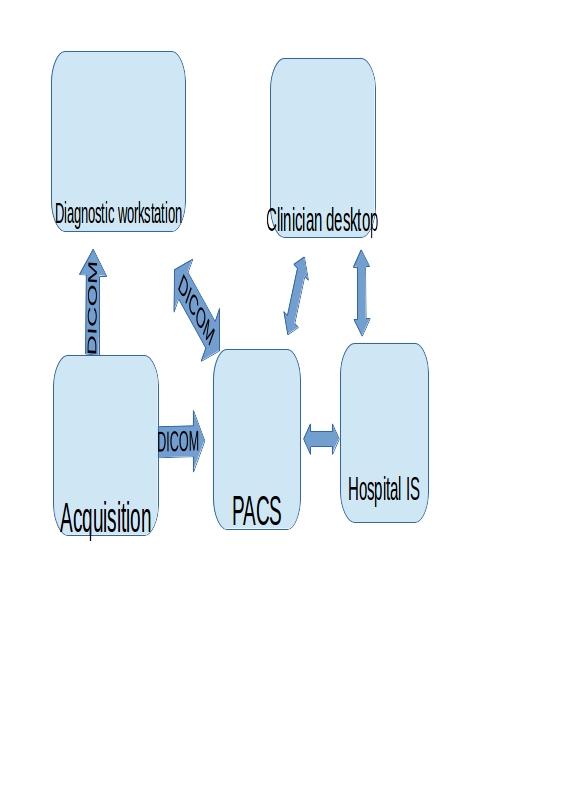
\includegraphics[width=0.8\textwidth, height=8cm]{chapter4/pacs.png}
    \caption{Typical workflow of medical image in hospital. Data acquisition is made by modalities (magnetic resonance, ultrasonography, X-ray radiography, etc.) and using DICOM format and protocol it can be directly transferred and visualized by diagnostic workstation. With metadata filled by an expert physician the image is stored in PACS. Other desktops within hospital can retrieve the image and review the report. The hospital information system may be involved in other workflows and communicate with other formats and standards (HL7,...)
    }
    \label{fig:pacs}
\end{figure}

As the data processed in hospital information systems contains sensitive information of real patients, these are protected and processing and storing is regulated by the national or international laws or agreements.
Development of telecomunication and network technologies a enabled telemedicine -- providing healthcare over remote distance. It requires to share and exchange  sensitive data of real patient among different helthcare providers and additionaly such data may be very valuable for further research. Security and encryption should be addressed and DICOM standard itself doesn't solve security issues appropriately, thus encyption during transferring the data over computer network must be ensured by other techniques.

In the Czech Republic, there exists several projects in production interconnecting different hospitals, clinics and other healthcare organization to exchange medical images. Project ePACS allows interconnecting each participant's PACS system via dedicated VPN channel to the central node and exchange of medical images are realized by routing the data flow from one VPN channel to the other\footnote{ePACS:\url{http://www.epacs.cz}, accessed January 2015}. Another approach is used in the project MEDIMED held by Masaryk University in Brno. Instead of dedicated VPN channel, they use  SSL encryption over standard TCP/IP communication and regional hospitals and healthcare providers are interconnected via the MEDIMED servers \cite{Slavicek2010,Zatloukal2012}.% \cite{Javornik2011,Zatloukal2012}.
In other countries, there were tested cross-border teleradiology in projects Baltic e-health, R-Bay and others \cite{Ross2010,Saliba2012}.
These projects are focused on sharing the medical images and other knowledge and information.

Storing the sensitive medical information is usually done in some trusted environment, e.g. in secured server or cluster owned by a trusted institution or within the hospital. In case of using distributed technologies, this lead to an idea to move and facilitate deployment of the grid services storing medical data to the institution which has been acknowledged to store them using e.g. pre-installed virtual machines as a sealed grid \cite{Kuba2007a}.

Additionaly for the research purposes an access to the wide range of medical images is needed for provenance, for research of new processing and diagnostic methods, etc.  DICOM records can be "deidentified" or anonymized for research purposes to protect sensitive personal data, but keep important information for research purposes. The Globus MEDICUS project published by Erberich et al.\cite{Erberich2006,Erberich2007} is based on Globus Toolkit middleware to federate clinical and research application via a grid-computing infrastructure. It  introduces a new DICOM Grid Interface Service for DICOM compliant devices and application based on Pixelmed Java DICOM Toolkit\footnote{\url{http://www.pixelmed.com/} accessed February 2015}. Currently the project is hibernated since 2008 and no further development was published\footnote{\url{https://dev.globus.org/wiki/Incubator/MEDICUS} accessed February 2015}. Similar effort was done with a project Medical Data Manager which uses gLite grid middleware by Duque, Montagnat et al.\cite{Duque,Montagnat2007} \footnote{\url{http://modalis.i3s.unice.fr/softwares/mdm/start} accessed February 2015} or MediGRID project by Krefting et al.{Krefting2009,Krefting2010}. These project focuses not only on sharing medical images and knowledge, but also on processing them using grid computing technologies\cite{Krefting2010}.

%When we look to the architecture of the systems of sharing medical images the problematic part within the point-to-multipoint architecture is the central part of the systems already in production e.g. in Czech Republic (MEDIMED, ePACS). This may become single point of failure and bottleneck.

To summarize this section, digital medical image acquisition, store, exchange and processing became common in the past years and is currently using distributed computing techniques. There are several efforts to implement medical data management within grid or cloud infrastructure for research purposes and integrate them with the production infrastructures. Security is solved by authentication, authorization mechanism as well as by encrypting the data and/or anonymizing them to keep minimal information useful for research. Thus there is another question, how easily the previously mentioned grid-based technologies can be integrated with current distributed systems used to integrate hospital PACS. The following section \ref{sec:methodsimages} describes methods used to integrate a pilot deployment of Globus MEDICUS with current regional system for exchanging medical images - MEDIMED. The realization and other promising particular results are described in section \ref{sec:resultsimages}.

\section{Methods to share medical images in grid}
\label{sec:methodsimages}

The integration strategies based on standard protocol integration and client server architecture is used to integrate Globus MEDICUS with some local PACS system. Globus MEDICUS \cite{Erberich2006,Erberich2007} implements a DICOM Grid Interface Service (DGIS) which in one side communicate using DICOM protocol, and implements other services which stores metadata and location of replicas of the data using standardized Globus toolkit middleware. DGIS behaves as a gateway to this grid infrastructure and is usually installed on the location of integrated third party system; hospital PACS, workstation PACS client or DICOM modality communicate with DGIS using DICOM protocol.
To present DICOM studies The integration strategy based on shared database or files can be used to present the DICOM studies via web portal. Additionally the web portal might generate specific DICOM queries to DGIS.

The paper \cite{kulhanek2009}  \emph{Processing of Medical Images in Virtual Distributed Environment} in Appendix \ref{app:a} published details about the integration of Globus MEDICUS instance with MeDiMed project with a conclusion that the integration via DICOM protocol is almost seamless. The paper \cite{Kulhanek2008Mefanet} presented additional portal integration with DICOMViewer, which can provide access to the DICOM studies available in the Globus MEDICUS infrastructure.


\section{Results}
\label{sec:resultsimages}
The pilot grid infrastructure was established in the location of First Faculty of Medicine, Charles University in Prague, Central Military Hospital in Prague and CESNET association. And the Globus Toolkit middleware and Globus MEDICUS implementation was installed on linux based virtual machines using XEN hypervisor providing pilot services to access this grid based PACS system.



%\chapter{Voice Science}
\label{sec:voice}
With introduction of objective data analysis and laryngoscopy methods the voice science emphasized the cooperation among  laryngologist, speech pathologist and voice teacher.
The human voice ranges from 50 Hz to something about 1000 Hz, but there are large  individual variation. For analysis of digitally recorded voice, either habitual or singing, the Discrete Fourier Transformation(DFT) is used to produce frequency and amplitude analysis of recorded input voice samples. One of the most used class algorithm to compute DFT is class of Fast Fourier Transformation with computational complexity $O(n \log(n))$ \cite{Cooley1965,Frigo2005} and parallel version of the algorithms may introduce additional speedup for larger samples of analyzed data \cite{Gupta1993,Takahashi2003}. The result of analysis can be visualized in a voice range profile and there can be seen significant difference between untrained and trained voice as well as quantitatively seen some disorders  \cite{DeLeoLeBorgne2002,wuyts2003effects}.

Other methods to analyse vocal chords is laryngoscopy. The videostroboscopy and high speed video in laryngoscope methods produce video for analysing the real movement of vocal chords. The videokymography method introduced by Švec et al. complements the videostroboscopy and allows to visualize and analyze movement of vocal cords recorded by high speed camera on standard TV or monitor with an artificial image built from recorded sequence of selected section \cite{Svec1996,Svec2007}. 

In case of recorded sound and further analysis there is a question about how such a service can be integrated in grid-computing or cloud-computing environment to provide access to a complex application for non-technical voice specialists. Additionally, the analytical software was already developed and calibrated for selected sorts of microphones in MS Windows platform \cite{Fric2007,Fric2012}. Therefore I proposed and implemented a method that provides access to the analytical software remotely. The section \ref{sec:methodsvoice} describes how the analytical software was customized with a remote desktop protocol (RDP). Results are described in section \ref{sec:resultsvoice}. Similar approach might be used for processing the video recordings from laryngoscope, however, the practical limits are discussed in section \ref{sec:conclusion}. 


\section{Methods for remote analysis of human voice}
\label{sec:methodsvoice}
%One method to provide access to specialized service is via remote access protocols. Secure Shell (SSH) is used to establish secure channel via unsecured network (e.g. the Internet) from SSH client to SSH server providing e.g. remote command-line, remote command execution etc. It is one of the basic method to access the grid infrastructure and submit computational jobs. 
%Another method is to have a web portal and this web portal based on user's input executes command-line batch scripts over SSH, or it can utilize web services to submit computational job.
Terminal access to some remote computational capabilities, e.g. remote command-line or remote execution is another integration strategy to some remote infrastructure. Secure Shell (SSH) is used to establish secure channel via unsecured network (e.g. the Internet) from SSH client to SSH server and it is basic method to access grid-computing infrastructure. 

Remote Desktop Protocol(RDP) is a proprietary protocol for desktop sharing developed primarly in Microsoft Windows platform, however, today clients and servers exists for several other platforms. Next to remote command-line, remote execution it allows to access remote graphical desktop environment. %VNC is sharing protocol to access remote graphical desktop environment\cite{Richardson1998}. 
The software for parameterized Voice Range Profile (ParVRP) and Voice Range Profile in Real time (RealVoiceLab) was already developed and calibrated for selected sorts of microphones in MS Windows platform by Fric et al.\cite{Fric2007,Fric2012}. The implementation is done in MATLAB environment utilizing Signal Processing Toolbox\footnote{\url{http://www.mathworks.com/products/signal/} accessed February 2015}and compiled with MATLAB Compiler and distributed as an executable.

Instead of migrating the application into some compatible platform for grid-middleware, a virtual machine was introduced and access to the software is provided via RDP protocol. RDP itself contains redirection of several services, e.g. sound recording or drive access. Because the default sound recording redirection introduces some sound degradation without control, I proposed, implemented and integrated the custom RDP plugin with the ParVRP and RealVoiceLab software to redirect the sound recording without loss of information. 

The computation of frequencies and amplitude from the recorded samples utilizes Fast Fourier Transformation which has time complexity $O(n\log(n))$. Thus the computational complexity and theoretical speedup is not primary reason for making such application distributed. 

This type of application can be packaged as virtual machine template and configured within different types of cloud infrastructures and together with a script or web portal the on-demand deployment can be automated.

\section{Results}
\label{sec:resultsvoice}

The paper \cite{kulhanek2010b} \emph{Remote Analysis of Human Voice--Lossless Sound Recording Redirection} in the Appendix~\ref{app:bio} published technical details and results of such implementation.

Additionally the custom RDP plugin with the ParVRP and RealVoiceLab software to redirect the sound recording without loss of information was packaged as a virtual machine template and  deployed in the pilot virtual infrastructure next to the test instance of Globus MEDICUS.

The virtual machine template was also deployed to different cloud computing infrastructures. One to the Amazon EC2\footnote{\url{http://aws.amazon.com/ec2/} accessed February 2015} and second to the pilot scientific cloud launched in the begining of 2012 --MetaCloud\footnote{\url{http://www.metacentrum.cz/en/cloud/} accessed February 2015}.

 A comparison of these two was presented to the users and staff of CESNET and EGI in EGI Technical Forum 2012\cite{Kulhanek2012a} with focus on providing such science as a service.
 
%\chapter{Computational physiology}
\label{sec:models}
A mathematical formalization of the fundamental knowledge and relation among biological system - mathematical model - is used as a base abstraction to utilize current discoveries of the genomics and proteomics and formalize the knowledge and construct a "Physiome Model". Model by it's definition is simplification of the complex reality.

Constructing the models and integrating them into complex entity which can be used for further purposes is schematically illustrated in fig. \ref{fig:modeling}. The measurements are done in laboratories or in hospitals. Lumped parameter models are usually represented as ordinary differential equations and differential algebraic equations and characterize the reality as topology of discrete elements. The imaging methods for processing and analysis (section \ref{sec:imaging}) are used to construct 3D models from segmentation and generating of mesh representation connected to physical principles. 
\begin{figure}[ht]
    \centering
    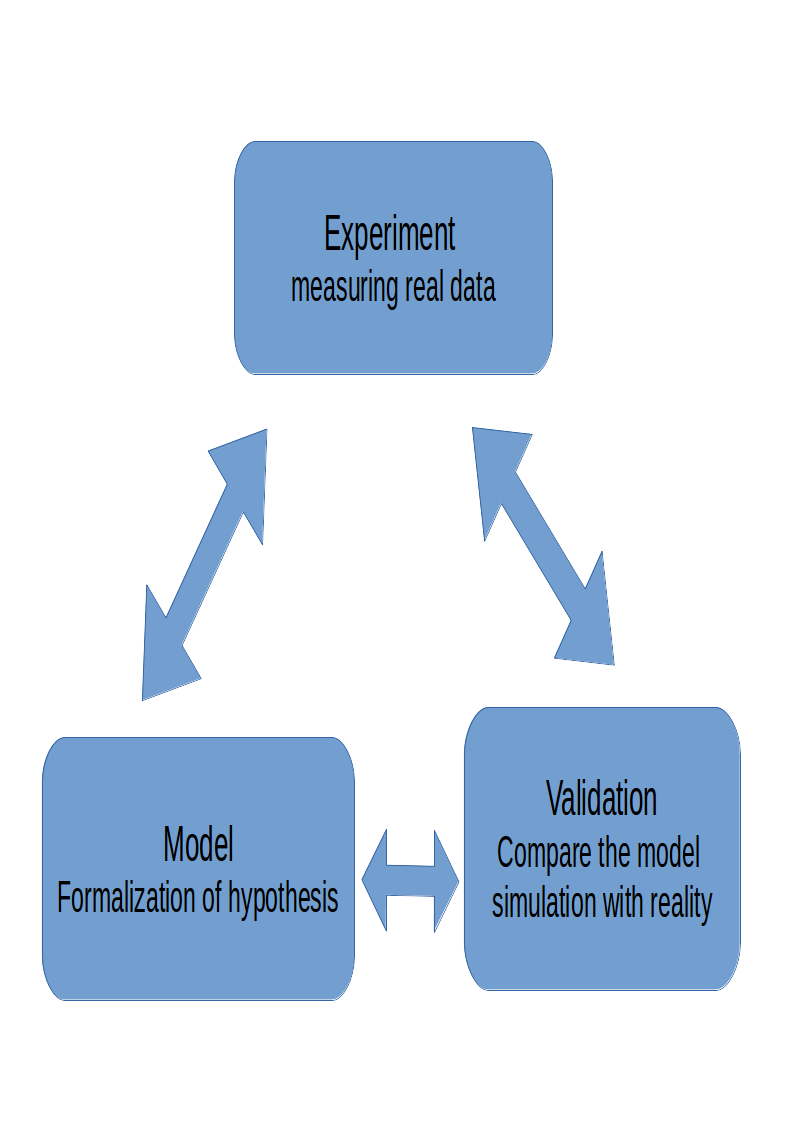
\includegraphics[width=0.5\textwidth, height=5cm]{chapter6/modeling.png}
    \caption{Schematic illustration of scientific process. The experiments produces data which are interpreted and hypothese is formalized as a model. Validation compares the model simulation with experiment, if model satisfies the criteria - is in agreement with real experiments, then the validated model can be used for other purposes.  %\bibentry{EGICompendium2013} \bibentry{egi2014}.
    }
    \label{fig:modeling}
\end{figure}

Application of the mathematical modelling techniques towards the biomedical research is sometimes called as systems biology approach combining the reductionism and integration as denoted by Kohl et al.\cite{Kohl2010}. Application towards the clinical praxis include the quantification of the diagnostic index or treatment strategy and it is a goal to develop tools, database models and methods of several Physiome projects, e.g. VPH-Physiome project presented by Hunter et al.\cite{Hunter2009}.

One of the earliest complex and integrative modelling effort was a model of circulation and it's regulation published by Guyton et al. in 1972 \cite{Guyton1972} which via derivative and technological upgrade continues as "Human Model" or "HumMod" introduced by Hester et al. \cite{Hester2011systems,hester2011} with a focus on integration effort. Different approach of modelling human physiology is a database of smaller models focusing on some particular physiological phenomenon. E.g. the NSR Physiome project introduces  JSIM\footnote{JSIM: \url{http://www.physiome.org/jsim/} accessed January 2015} Java based simulation system to support modeling in  physiology. Repository of several hundred of models were published using this system \cite{Butterworth2014}. The similar effort is done by IUPS Physiome project and repository of models are  based on XML standard languages CellML and FieldML \cite{Hunter2004,Yu2011}. The Systems Biology Markup Language (SBML) is used for modeling biological system at the level of biochemical reaction and regulatory network and another database collects several hundreds of curated and non-curated models \cite{Hucka2004,LeNovere2006}.

JSIM, CellML, SBML or HumMod are domain specific languages and the tools able to work with them are primarily developed within physiological or systems biological communities. Other authors use commercial or industry standard tools for mathematical modelling and computing. E.g. Kofranek et al. describes Guyton's 1972 model in MATLAB\textsuperscript{\textregistered} Simulink \cite{Kofranek2010} and the derivative HumMod in acausal object-oriented Modelica language \cite{Kofranek2011hummod,kofranek2013hummod}. Fernandez et al. describes models of cardiovascular pulsatile system using MATLAB Simscape  \cite{FernandezDeCanete2013} and recently in Modelica  \cite{FernandezdeCanete2014}.

Thus there is an open debate whether in-house domain specific language and tools like JSIM, CellML and FieldML,SBML or HumMod reached it's capabilities for representing complex models. Only the HumMod reached the integrative approach building the complex integrative model of human physiology using lumped parameter approach. I contributed to the idea of key features which involves acausal modeling technique and object orientation which keeps the complex model structure decomposed into understandable and maintainable parts and allows to cover complexity of models like HumMod. 

The methods and examples of modeling cardiovascular system are described in the next section \ref{sec:methodsmodels}. The methods of estimating parameters of complex models are described in section \ref{sec:methodsestimation} and particular results are described in section \ref{sec:resultsestimation}.

%\label{sec:results}
\section{Modeling methodology}
\label{sec:methodsmodels}
%For building complex models it seems that acausal (or declarative) modeling technique is key feature as it allows to express the variables declaratively, acausal modeling tool (e.g. Modelica or MATLAB\textsuperscript{\textregistered}  SIMSCAPE\texttrademark) figures out which are the dependent and independent variables upon compilation\cite{fritzson2002}. This allows building complex systems of equation from composed components and the model diagrams still captures the essence of the modeled reality much better and the simulation models are much more legible and thus also less prone to mistakes\cite{Kofranek2008,FernandezDeCanete2013}. 
The methodology of formalizing mathematical models is influenced by the abilities of underlying modeling language used. %As it was noted in previous chapter \ref{sec:intromodels}, the technology used for formalizing mathematically knowledge may introduce some benefits.
%\subsection{Modelica}
The Modelica language is an object-oriented, equation based and acausal modeling language standardized by Modelica association\footnote{\url{http://www.modelica.org} accessed February 2015}.

Object orientation means that the definition of model is class as in object oriented programming, instance of the model is object,  each instance can share type and differ in parameters and the place where it is used, inheritance and some sort of polymorphism is possible.

Equation based means that the equation is not statement, thus the relation among variables can be expressed in any form. Modelica tool will decide which one is input and output upon compilation. E.g. from the equation $q = \frac{dV}{dt}$ the process of computation can lead to $ q:= der(V)$ or $ V := \int{q}dt$ based on whether the $V$ or $q$ is known from the context.

Acausal connector is special purpose class to define variables of the model shared with other models or classes. Connecting two or more components via acausal connector will generate equality of all "non-flow" variables in connected connectors: $$p_1=p_2=\ldots =p_n$$
and zero sum of all "flow" variables $$ \sum_{i=1}^n q_i=0$$

%As an example, we will declare components important for modeling cardiovascular system (CVS). The components are hydraulic elastic ballon, which is analogy of electrical capacitor, and hydraulic resistor, analogy of electrical resistor.
%
%Connector \emph{HydraulicPort} with "flow" variable $q$ and non-flow variable pressure $p$ is presented in Modelica source code:
%\begin{lstlisting}[language=modelica]
%connector HydraulicPort
%  flow Real q;
%  Real p;
%end HydraulicPort;
%\end{lstlisting}
%
%Model of hydraulic resistor(conductor) with parameter $G$ denoting conductance and two hydraulic ports express the equations:
%\begin{equation}
%q_{in}.q = -q_{out}.q \label{eq:conductor1}
%\end{equation} 
%\begin{equation}
% q_{in}.q = G \times (q_{in}.p-q_{out}.p) \label{eq:conductor2}
%\end{equation}
%presented in Modelica source code:
%\begin{lstlisting}[language=modelica]
%model HydraulicConductor
%  parameter Real G;
%  HydraulicPort qin;
%  HydraulicPort qout;
%equation 
%  qin.q= -qout.q;
%  qin.q = G*(qin.p-qout.p);
%end HydraulicConductor;
%\end{lstlisting}
%
%
%Model of hydraulic elastance with parameters $V_0$ as unstressed volume $p_0$ external pressure and $C$ compliance(reciprocal value of elastance) with state variable $V$ volume express these equation:
%\begin{equation} \label{eq:compliance}p-p_0 = \left\{   
%  \begin{array}{l l} 0 & \quad \text{if } V \text{\textless} V_0 \\ 
%    \frac{V-V_0}{C} & \quad \text{otherwise}
%  \end{array} \right.\end{equation} 
%\begin{equation}\label{eq:flowrate}\frac{{\rm d}V}{{\rm d}t} =  q\end{equation} 
%is presented in Modelica source code:
%\begin{lstlisting}[language=modelica]
%model HydraulicElastance
%    Real V;
%    parameter Real V0;
%    parameter Real p0;
%    parameter Real C;
%  HydraulicPort qin;
%equation 
%   qin.p -p0 = if (V<V0) then 0 else (V-V0)/C;
%   der(V) = qin.q;
%end HydraulicElastance;\end{lstlisting}

The paper \cite{Kulhanek2014Modeling} \emph{Modelling of Short-term Mechanism of arterial pressure in the cardiovascular system: Object-oriented and acausal approach} in Appendix~\ref{app:d} published disputation about causal and acausal approach in using Modelica for modeling lumped parameter CVS model. 

The paper \cite{Kulhanek2014mefanet} \emph{Simple Models of the Cardiovascular System for Educational and Research Purposes} in Appendix~\ref{app:simplemodelsd} published detailed methodology of modeling pulsatile CVS in Modelica. 

Comprehensive guide to the Modelica language and it's capabilities are in the book of Fritzson \cite{fritzson2002} or in the on-line book by M.Tiller \cite{Tiller2014}.

\section{Parameter Estimation}
\label{sec:estimation}

%\subsection{Identification of physiological systems}
%Model verification (whether simulation of the model shows desired behavior) and model validation (whether model simulation agrees with new observation of real system) are important steps in system analysis and model construction. 
Usually some knowledge of the system - the structure is available and unknown coefficients (parameters) remain unknown. Once the model is formalized and constructed, further problem is to estimate the model parameters so that the model reproduces real world system. This procedure is sometimes called model identification \cite[p.~159]{khoo2000}. The objective of this task is usually to minimize the following function (to find least squares of the differences between predicted and measured values):
\begin{equation} \label{eq:parameter} 
f( \vec{p} ) = \sum_{i=1}^{n} ( M(t_{i},\vec{p} ) - d(t_{i}) )^2 \to min  
\end{equation} 
where $\vec{p}$ is vector of values of parameters, $M(t_{i},\vec{p})$ is model simulated at time $t_{i} $ with the given parameter values $\vec{p}$ and $d(t_{i})$ is the measured experimental value at time $t_{i}$.
Algorithmically, this problem was shown to belonging to the \emph{NP-complete} problems \cite{Hofmann2005} thus the best exact algorithm is based on brute force search - trying all possible values of parameters and simulate the model with them and find minimum of the objective function \ref{eq:parameter}. 
However, exact solution may not be needed because the models itself are by definition approximation of real system, and the input data are measured with some degree of error. 
As in other problems where exact algorithm uses brute-force search, some heuristic or randomization method should be used for bigger space of potential input data. 
After the parameter estimation a further problems arise with structural identifiability and analysis of sensitivity to the estimated parameter values\cite[p.~176]{khoo2000}. 

Parameter estimation and further analysis methods are part of specialized mathematical software. E.g. Pruet et al. used Metropolis algorithm to produce a distribution of parameters to calibrate the model of human cardiovascular physiology, which were further tested against predictive ability of circulatory failure and statistical methods performed in the software Wolfram \textit{Mathematica} \cite{Pruett2013}. The iterative improvement method in the software MATLAB Simulink\textregistered ~was used in estimating 2 parameters of simple cardiovascular model by Takahashi et al. \cite{Takahashi2013}. Several methods were compared in estimating multiple parameters of cardiovascular system in MATLAB Simulink\textregistered ~by Abbass et al. \cite{Abbass2012}.

Heuristic methods reduce the number of simulation and additionally some set of  simulation can be computed concurently e.g. in grid or cloud computing infrastructure. 
Maffioletti et al. published GC3Pie framework utilizing evolutionary algorithms and introduced workflow to identify parameters of models for economical predictions using grid computing \cite{maffioletti2012computational}. Humphrey et al. calibrated hydrology models utilizing commercial Windows Azure cloud computing infrastructure with a significant speedup on the modified dynamically dimensioned search algorithm\cite{Humphrey2012,Tolson2007}. 

%Selected methods to estimate parameters are introduced in section \ref{sec:methodsmodels}. 

As already identified also by other authors of some calibrating systems, the parameter estimation is used sporadically, however, with high demand of computational task in temporal time. Thus, I proposed and designed the system which can distribute the simulation task into grid-computing and cloud-computing infrastructure and the computational capacity can be provisioned on-demand.% this brings significant speedup for parameter estimation of complex model but limited speedup on simple models. 
Methods are described in section \ref{sec:methodsestimation} and interesting results are described in section \ref{sec:resultsestimation}.

\section{Methods for Parameter Estimation}
\label{sec:methodsestimation}
Evolutionary algorithms are used for finding global minimum or maximum and it can be used to estimate the parameters of the model. Genetic algorithm is type of evolutionary algorithm and the general structure of the algorithm is presented in figure \ref{fig:GA-kopenogram}.

\begin{figure}[htb]
    \centering
    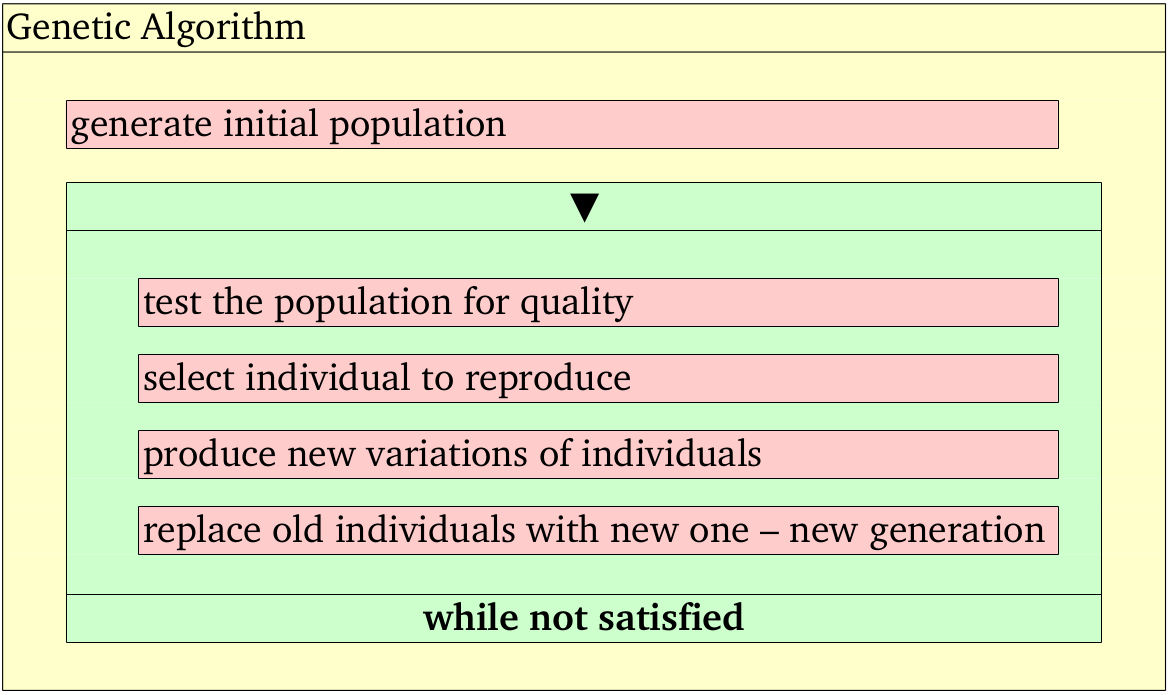
\includegraphics[width=0.6\textwidth]{chapter6/GA-kopenogram.png}
    \caption{General structure of genetic algorithm presented as kopenogram. Kopenograms are graphical language for structured algorithms to supplement UML proposed by Kofranek et al.\cite{Kofranek2012}.
    }
    \label{fig:GA-kopenogram}
\end{figure}


\begin{figure}[htb]
    \centering
    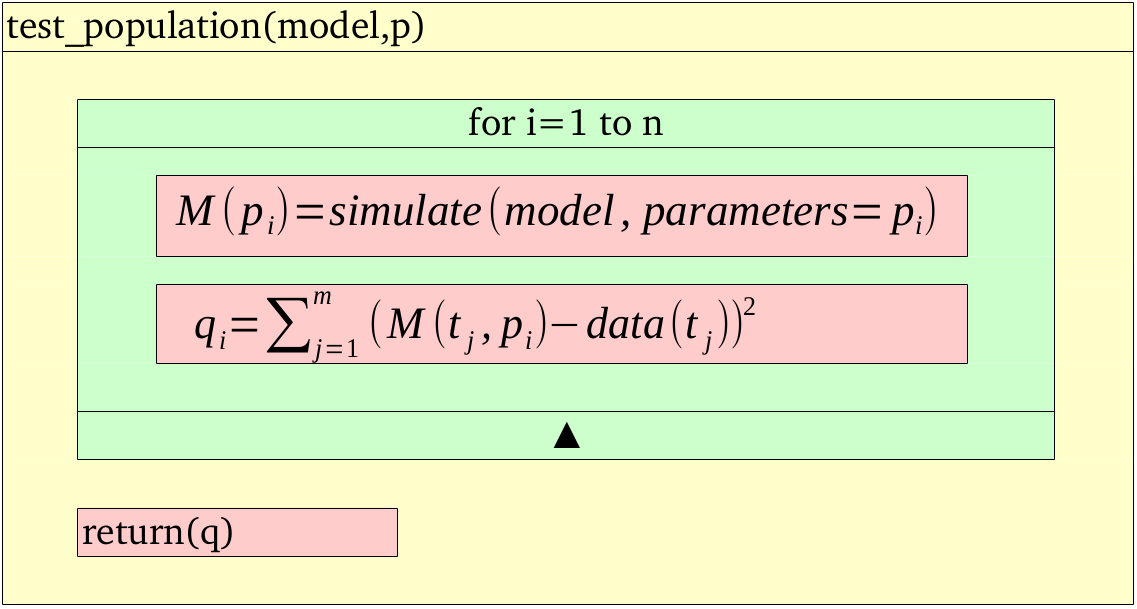
\includegraphics[width=0.6\textwidth]{chapter6/GA-kopenogram2.png}
    \caption{Specific test of the population for quality in case of parameter estimation. Model is simulated according to individual $i$ with parameters $p_i$ and the quality $q_i$ is counted per the objective function \ref{eq:parameter}.
    }
    \label{fig:GA-kopenogram2}
\end{figure}

The iteration within the loop "$\blacktriangledown \ldots$ \emph{while not satisfied}" depends on previous iteration, thus in general it cannot be parallelized.
In the case of parameter estimation, the step \emph{test the population for quality} has algorithmical structure as in fig.\ref{fig:GA-kopenogram2}. Each iteration in the loop "\emph{for i=1 to n}" is independent and a therefore loop parallelism (section \ref{sec:parallelprogramming}) can be utilized and implemented here.

The Amdahl's law in equation \ref{eq:amdahl} can be used to estimate  the theoretical speedup limitation for the specific model and potential gain for identifying different types of models can be stated. We assume that the simulation of the model with any parameters will take the same time, even this is not generally true as the non-linear models and numerical methods may cause different steps to be performed for different parameter values. 

The specific fraction $\alpha$ for the model determines the level of scalability of the model within the parallelized system. For the complex models the $\alpha$ will decrease. The specific estimates of the fraction $\alpha$ and it's influence on the scalability and results are presented in section \ref{sec:resultsestimation}.

\subsection{Architecture of system for parameter estimation}

The architecture of the system implementing the algorithms in fig. \ref{fig:GA-kopenogram} and \ref{fig:GA-kopenogram2} will determine the overhead which may affect significantly the computation time.

The architecture of the proposed system is in fig \ref{fig:architectureestimation}.
\begin{figure}[htb]
    \centering
    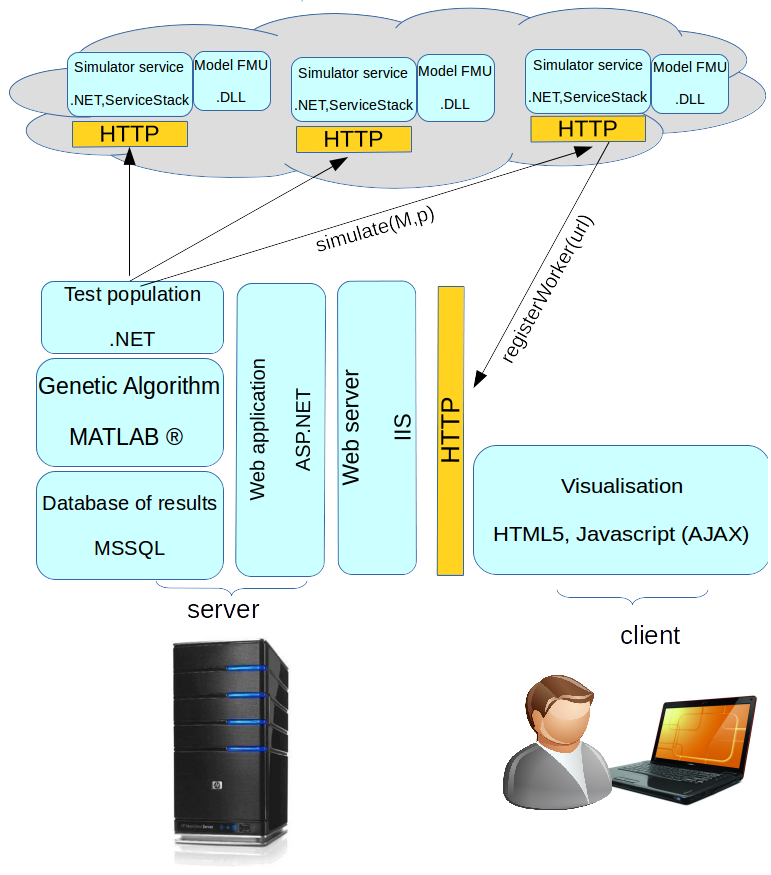
\includegraphics[width=0.6\textwidth]{chapter6/architekturaestimation.png}
    \caption{Architecture of the system employing genetic algorithm and concurent simulation of models in cloud.
    }
    \label{fig:architectureestimation}
\end{figure}
Modelica models can be exported as proprietary C/C++ code or binary EXE with some default command-line options to perform simulation. Modelica models can be exported into standard Functional Mockup Unit(FMU) with is standardized XML metadata packaged together with  binary library .DLL (or .SO) following standardized API\footnote{\url{https://www.fmi-standard.org/} accessed February 2015}.


\section{Results}
\label{sec:resultsestimation}

The paper \cite{Kulhanek2014Parameters} \emph{Parameter estimation of complex mathematical models of human physiology using remote simulation distributed in scientific cloud} in Appendix~\ref{app:c} published the architecture and results achieved on estimating parameters on three  different types of models from the non-complex, medium-complex and complex model.

\section{Results}
\label{sec:results}
In previous chapters, there were introduced different methods available for selected use cases in research in biology and medicine. 
%\section{Virtual Infrastructure}
%\label{sec:resultsinfrastructure}
As each of the use cases and available system was proposed on different operating system platform, different architecture and or different middleware the virtualization was utilized to build the virtual infrastructures for purposes of each project. The paper \cite{kulhanek2010c} \emph{Infrastructure for Data Storage and Computation in Biomedical Research} in Appendix~\ref{app:infrastructure} describes result of establishing the virtualization on physical infrastructure to share computational power among different platforms.
 %results
\section{Conclusion}
\label{sec:conclusion}

\section{Discussion}
%Important decision about utilizing distributed computing infrastructure is what benefits it'll bring with respect of the caveats and resources it'll consume including the human capital compared to other existing solution.

%\subsection{Medical imaging}
%There are several use cases where exchanging or sharing DICOM images are beneficial, next to the second opinion and teleradiology (remote diagnostics), gathering information and expertize in rare diseases, studies in unusual cases or secondary use of clinical imaging data for research, optimizing new processing methods etc. 

%The Globus MEDICUS stores one or more copies of DICOM images within grid infrastructure, and as such, can be used as technology and infrastructure to built data warehouse for DICOM images of specific interest. Another philosophy is to federate files and metadata stored within home institutions, which seems to be preferred solution in hospitals and clinical use which were shown in other medical sharing image projects.

The result presented in section \ref{sec:resultsimages} is an example how a standard format and protocol (DICOM) is utilized to integrate current production system to exchange medical images (MEDIMED) and a grid based solution (Globus MEDICUS) where an underlying technology is hidden for common user. This research was originally motivated by the idea to investigate benefits and show robust grid-based technology against proprietary distributed technology, which may face up to scalability and maintenance issues. Another issue is the philosophy of storing medical images. The presented solution based on the Globus MEDICUS is in general a data warehouse storing one or more copies of DICOM images, in contrast to federated files and metadata stored within home institutions which shares only network infrastructure to interchange the DICOM studies. This seems to be more acceptable by hospitals and by the national and international regulation for clinical and diagnostic use, e.g. The authors of Globus MEDICUS in their further development followed a way of federation of medical images stored within home institutions rather than in a grid infrastructure published by Chervenak et al. \cite{Chervenak2012}. 
Thus the grid-computing infrastructure for sharing medical images is worth to use in the cases when additional demanding computation e.g. for processing of medical images are needed or for educational, training and knowledge sharing purposes.

%However, the scalability is managed within the current MEDIMED system and separate PACS system including database of anonymized medical images with the medical context and description for research and education purposes coexist within the current system.


%This allows to keep current tools for processing the medical images when the technology of infrastructure is changed.
%Thus user experience is kept on using same tools or same workflows, however, accessing much broader database of records or having more powerful tools for processing the data.
 
The majority of user experience is kept also in the case of the application of remote voice analysis presented in section \ref{sec:resultsvoice}. The processing/analyzing application was kept on it's original platform but moved to remote server and a remote desktop protocol is used to redirect interaction and voice recording from user's computer to remote server and vice versa. Manipulating the . The recordings are stored on remote server for secondary use for further research and analysis algorithm improvement and in case of growth, the long-term storing issue of scientific data will be needed as in the case of medical images. Such kind of service can be deployed on any web server and a occasional need to educate or perform higher number of analysis concurently can be satisfied with cloud-computing deployment 

In the case of application for parameter estimation presented in section \ref{sec:resultsestimation} the user must fill the data in a form that is a spreadsheet like table and respecting some simple convention. As seen from results, the computation is sensitive on communication overhead therefore more high performance computing (HPC) hardware would be beneficial for such computation. However for medium and highly complex models the deployment of worker nodes into cloud-computing environment to for virtual HPC cluster is worth to consider. The application for parameter sweep is embarassingly parallel and suitable for high throughput computing (HTC) which is the main focus of current grid-computing infrastructures.   
%The added value of the grid-computing or cloud-computing technology is the ability of enhanced collaboration in use cases which were difficult to achieve, e.g. in cases if secondary use of clinical imaging data for research

%for is an important area in research of rare diseases. As seen from the results obtained either in previous chapter or by other authors, the grid-computing is only one technology to facilitate some interconection of storage and computation capacity of different sites and servers owned by different organizations or individuals. 

%As seen from the results, there are several main purpose for which the grid-computing or cloud-computing infrastructure was built and are currently used for:
%\begin{enumerate}
%\item{solve big computational problems in distributed environment and achieve results in a reasonable computational time}
%\item{facilitate processing of the computation to support processing, analysis for further scientific results. This is provided by scientific portals, services, workflows etc. which allows non-exports in grid-computing or cloud-computing to do their job reducing researcher's time.}
%\item{share and archive database of scientific data for further processing and reproducibility.}
%\end{enumerate}
%\subsubsection{Scalability}
%
%From the perspective of efficiency (time complexity) and scalability (degree of parallelization) the heuristic methods for parameter estimation application brings at least some solution in a reasonable time. For small models it, however, doesn't make sense as the overhead and parallelizable fraction limits the speedup gain from distribution to grid or cloud-computing\ref{sec:resultsestimation}. 
%
%For complex models the infrastructure of grid-computing or cloud-computing can be used to distribute simulation tasks to explore wider space of possible solution.

\subsubsection{Platform}

One of the important decision when porting an application to the grid environment is the platform of the used system. %The service-grid 

The architecture which involves computational nodes deployed in cloud-computing infrastructure was influenced by the fact, that the model implementation is exported from third party tool to the standard FMU library as mentioned in section \ref{sec:methodsestimation} for the MS Windows platform, which determines the platform of the worker node. The virtualization - or in case of parameter estimation a cloud computing is utilized on prepared platform with MS Windows Datacenter license. In case of parameter sweep a desktop-grid computing BOINC worker and application for MS Windows platform only is prepared for volunteers with the compatiblet system. 

To utilize service-grid infrastructure an export of the model into FMU library and implementation of the wrapper service should be done in the grid-computing platform which is usually Linux based system. Another option could be to use WINE\footnote{\url{https://www.winehq.org/} WINE. Accessed March 2015} -- compatibility layer capable of running Windows applications on several POSIX-compliant operating systems, such as Linux, Mac OSX, BSD. 

%With respect to scalability the degree and fraction of paralelization from the whole computational process needs to be considered, as, e.g. for simulating simple models and estimating the parameters takes couple of minutes to hours on single computer, which may be acceptable and deployment on grid computing will introduce overhead which degrades the benefits.

\subsubsection{Porting}
Each of the introduced systems and application was from it's beginning prepared for serial workflow. To achieve higher level of programming model,  some manual intervention is usually needed on the system or source code of application.

For the smaller types of application and scientific community with their own tools it is the question, whether to invest on porting their tools to grid specific platform and parallel programming model. In the case of voice science, the analytical application was deployed on virtual machine and made available via remote desktop feature. This caused that users and researchers may stay at their platform and focus on their key technologies and research rather than to learn new one.

For the case of algorithms, that are already present in grid-computing middleware is key factor the worker/simulation part which is specific for each research community. 

%The infrastructure built for purpose of large projects becomes open for smaller teams of scientists who doesn't have strong IT department or background. The process introduced before might be inneficient in terms of researcher's time who may spent time to porting it's application and tunning it up in grid or cloud environment. 

%Integration to tools researchers already use, or introduce new tools with low learning curve ...



%It was also shown that the batch-processing is not appropriate for some sort of application. The voice analysis is expected to be done in real-time and with access to some additional software, services and databases which are hard to maintain locally. 

\section{Future work}
%\subsubsection{Long Tail Science}

The "long-tail" movement described by Anderson \cite{Anderson2006} is business strategy of companies such as Amazon and Apple focusing on offering and delivering not only very popular products but also products with relatively small quantities sold each to final consumers in a price acceptable for them  due to reduced sales, marketing and delivery costs. The expansion of Internet and it's related technologies caused this strategy to be profitable and successful and sales of minor products outperforms the most popular products .

%The provenance and reproducibility of scientific results implied a need to long-term preservation of scientific data, however, if it is left on individual researcher, there is loss of data, as analysed by Vines et al. or Heidorn \cite{Vines2014,P.BryanHeidorn2008}.
 
There is a discussion about how to preserve the scientific data in a long-term way to prevent loss of them  \cite{Vines2014,P.BryanHeidorn2008} and to facilitate an access to computational resources for large amount of small scientific groups which have limited resources to port, integrate or customize their current tools and processes -- the so called long-tail of science. Cloud-computing technologies seems to be customizable and may be an enabling technology to focus on long-tail science consumers as noted e.g. by Weinhardt et al.\cite{Weinhardt2009}. The future work in this area may contribute to design and implement policies for long-term scientific data storage and service available for them to gain access to the powerfull capacity of grid-computing and cloud-computing infrastructure. 

The medical imaging and processing methods are used to identify the parameters of models of human physiology for further diagnosis statement and treatment decision. E.g. Ralovich et al.\cite{Ralovich2012} proposed a noninvasive method based on computational fluid dynamic and magentic resonance imaging (MRI) to identify pressure difference in aorta for further hemodynamics analysis based on four element windkessel model. However, such type of studies usually focus on particular phenomenon and tries identify parameters of very simplified models that are currently known in systems biology domain. In the time of writing this thesis, Magnetic Particle Imager \footnote{introduced first by Gleich and Weizenecker\cite{Gleich2005}} (available only for animal models and not yet for human medicine) can produce high resolution images with fast shutter speed (~20 ms). Several computational and storage demanding biomedical application were shown in animal models by Saritas et al.\cite{Saritas2013}. There are research infrastructures which were established to coordinate the research in biology and medicine, e.g.   Integrated Structural Biology Infrastructure for Europe (INSTRUCT)\footnote{\url{https://www.structuralbiology.eu/} accessed March 2015}, European Life Science Infrastructure for Biological Information (ELIXIR)\footnote{\url{http://www.elixir-europe.org/} accessed March 2015},  European Biomedical Imaging Infrastructure (Euro-BioImaging)\footnote{\url{http://www.eurobioimaging.eu/} accessed March 2015} and others. As noted by Hunter et al.\cite{Hunter2013} the purpose of these initiatives is to understand high-level phenotypes from genomic, metabolomic, proteomic, imaging and other types of data which requires multiscale mathematical models and simulation deli4vered e.g. by virtual physiological human (VPH)\footnote{\url{http://www.vph-institute.org/} accessed March 2015} project. 
%And the grid-based or  cloud-based medical data management solution can be used as technology and infrastructure to store and share the expected big ammount of raw scientific results, such as images or videos. 

The integration with multidimensional models of geometrical, mechanical properties and the time-dependence of the compartments data taken from the medical and biological repositories is a challenge for current "physiome" projects. Current complex models of human physiology are based mainly on lumped parameter approach, some of the compartments are described by physical or chemical laws, while others are only empirically determined curves described by parameters which doesn't have further physiological meaning and can't be measured.  Future direction of research may focus on integrative effort of the multiscale modeling which may improve an effort towards patient specific health care, in silico trails and drug discovery.   %Some of the methods and pilot results were shown in sections \ref{sec:resultsestimation} and \ref{sec:resultsboinc}. 

\section{Summary}

This thesis presents the infrastructure which thanks to virtualization technology joined several domain specific tools in the field of sharing and processing medical images, performing real-time voice analysis and simulating human physiology.  

A seamless integration of grid-based PACS system was established with current distributed system to share DICOM medical images. An access to real-time voice analysis application via remote desktop technology brings this type of service to any computer capable to connect to Internet. A system to support analysis and building complex models of human physiology in the phase of parameter estimation and parameter sweep was introduced and additional computational nodes can be flexibly joined by starting prepared virtual machines in cloud-computing deployment. Methodology of building complex models of human physiology was contributed with the idea of acausal and object-oriented modeling techniques.
 %discussion,conclusion

\bibliographystyle{unsrturltom}
\bibliography{bibliography/Dizertace}
\chapter{Infrastructure for data storage and computation in biomedical research}\label{app:infrastructure}
The paper \cite{kulhanek2010c} published as
 
\bibentry{kulhanek2010c}

\end{document}
